\documentclass[12pt]{article}

% UTF-8 encoding and fonts
\usepackage[utf8]{inputenc}
\usepackage[T1]{fontenc}
\usepackage{lmodern}

% Page setup
\usepackage[margin=1in]{geometry}
\usepackage{setspace}
\onehalfspacing

% Typography
\usepackage{microtype}

% Math and symbols
\usepackage{amsmath,amssymb}

% Graphics
\usepackage{graphicx}
\usepackage{float}
\usepackage{subcaption}

% Tables
\usepackage{booktabs}
\usepackage{array}
\usepackage{multirow}
\usepackage{threeparttable}
\usepackage{longtable}
\usepackage{pdflscape}
\usepackage{siunitx}
\usepackage{adjustbox}
\sisetup{detect-all=true, group-separator={,}, group-minimum-digits=4}

% Bibliography
\usepackage{natbib}
\bibliographystyle{aer}

% Hyperlinks
\usepackage{hyperref}
\hypersetup{
    colorlinks=true,
    linkcolor=blue,
    citecolor=blue,
    urlcolor=blue
}
\usepackage[nameinlink,noabbrev]{cleveref}

% Timing data
\IfFileExists{timing_data.tex}{\input{timing_data.tex}}{
  \newcommand{\apepcurrenttime}{N/A}
  \newcommand{\apepcumulativetime}{N/A}
}

% Captions
\usepackage{caption}
\captionsetup{font=small,labelfont=bf}

% Section formatting
\usepackage{titlesec}
\titleformat{\section}{\large\bfseries}{\thesection.}{0.5em}{}
\titleformat{\subsection}{\normalsize\bfseries}{\thesubsection}{0.5em}{}

% Custom commands
\newcommand{\E}{\mathbb{E}}
\newcommand{\sym}[1]{\ifmmode^{#1}\else\(^{#1}\)\fi}

\title{Going Up Alone: Automation, Trust, and the Disappearance of the Elevator Operator}
\author{APEP Autonomous Research\thanks{Autonomous Policy Evaluation Project. Correspondence: scl@econ.uzh.ch{} (cumulative: \apepcumulativetime{}).} \and @SocialCatalystLab}
\date{\today}

\begin{document}

\maketitle

\begin{abstract}
\noindent
Why did elevator automation---technically feasible from 1900---take over forty years to achieve widespread adoption? We document the complete lifecycle of the only occupation in the U.S. Census ever fully eliminated by automation: the elevator operator. Using full-count census microdata covering 680 million person-records (1900--1950) and 73.7 million linked individual records, we show that operator employment grew tenfold from 7,943 to 82,666 despite the technology's availability. Synthetic control analysis of the 1945 New York City elevator operator strike reveals a paradox: the strike's epicenter retained operators longer than comparable jurisdictions over the subsequent decade, suggesting that the coordination shock reinforced rather than displaced the local workforce. Tracking 38,562 individual operators longitudinally, we find that only 15.8\% of the 1940 cohort remained in the occupation by 1950, with sharp racial and geographic disparities in transition outcomes.
\end{abstract}

\vspace{1em}
\noindent\textbf{JEL Codes:} J23, N32, O33, J51 \\
\noindent\textbf{Keywords:} automation, technology adoption, behavioral frictions, elevator operators, occupational displacement, synthetic control

\newpage

\section{Introduction}

In 1940, the United States Census recorded 82,666 elevator operators---men and women whose sole job was to ferry passengers between floors by manually operating a lever. By 1970, the occupation had functionally ceased to exist. The elevator operator is the only occupation out of 270 tracked in the 1950 Census Classification to be entirely eliminated by automation \citep{bessen2016}. Every other occupation that shrank was absorbed, renamed, or consolidated. Elevator operators simply disappeared. Our data captures the critical decade of the transition: between 1940 and 1950, the absolute count barely grew (to 85,294), but the rate per employed worker fell for the first time in the occupation's history---the structural break that would accelerate into complete elimination by 1970.

The puzzle is not that the occupation died. The puzzle is that it lived so long.

Automatic push-button elevators were demonstrated in the early 1900s. By the 1920s, the Otis Elevator Company had developed reliable self-service systems. By the 1930s, building owners could calculate that eliminating the operator's wage would pay for the retrofit within months. Yet the occupation \textit{grew} relentlessly: from 7,943 operators in 1900 to 23,376 in 1910, 36,437 in 1920, 62,676 in 1930, and 82,666 in 1940. Four decades of technological readiness produced not adoption but expansion.

The barrier was not cost. It was trust. Riders refused to enter an elevator without a human operator. Building owners who installed automatic systems faced tenant complaints, vacancy, and even legal liability. The result was a coordination failure: no individual building owner wanted to be first to remove operators, even though all would benefit from the transition. A superior technology sat dormant because the equilibrium---human-operated elevators---was self-reinforcing.

This paper makes three contributions. First, we construct the first comprehensive empirical atlas of a fully automated occupation, using IPUMS full-count census microdata spanning six decennial censuses (1900--1950) and covering over 680 million person-records \citep{ruggles2024}. We document the occupation's rise, its demographic transformation---feminization from 1.5\% to 30.9\% female, persistent racial stratification at roughly one-quarter Black, and dramatic aging of the workforce---and its sharp geographic concentration, with New York alone accounting for over one-third of all operators.

Second, we use the September 1945 New York City elevator operator strike as a natural experiment to study how coordination shocks interact with local institutions. For six days, 15,000 striking operators forced 1.5 million office workers to walk stairs or experience minimal-service elevators. Within a decade, the automated share of new elevator installations surged from 12.6\% to over 90\%. Using synthetic control methods \citep{abadie2010, abadie2015}, we compare New York State---where the strike was concentrated---to a data-driven counterfactual over the 1940--1950 decade. Paradoxically, we find that the strike's epicenter \textit{retained} operators at higher rates than the synthetic counterfactual ($p = 0.056$), consistent with union contracts and political backlash reinforcing the occupation locally. We interpret this as suggestive evidence that coordination shocks can have heterogeneous local effects, though we acknowledge the limitations of decennial data and a design that effectively relies on a single comparison unit (Washington, D.C.).

Third, we track individual elevator operators across the 1940--1950 decade using the IPUMS Multigenerational Longitudinal Panel (MLP) v2.0 crosswalk \citep{ruggles2021}, which links 73.7 million individuals across consecutive censuses. Among 38,562 linked elevator operators (46.7\% linkage rate), we construct complete occupational transition matrices documenting where workers went. Only 15.8\% remained elevator operators by 1950. The largest shares transitioned out of the labor force entirely (16.4\%), moved into operative/manufacturing work (12.7\%), became craftsmen (12.2\%), or shifted to farm work (11.0\%). These comparative transition patterns---descriptive rather than causally identified---reveal significant heterogeneity by race, sex, age, and geography, with Black operators and older workers facing markedly worse transition outcomes.

This paper speaks to several active literatures. Most directly, it contributes to the economics of automation and labor displacement. \citet{acemoglu2020} document the negative employment effects of industrial robots; \citet{acemoglu2019} develop a task-based framework for understanding how automation displaces and reinstates labor; \citet{autor2003} measure the skill content of technological change. Our contribution is to study the \textit{only} case of complete occupational automation, providing a limiting case for these theories.

We are closely related to but fundamentally distinct from \citet{feigenbaum2024}, who study the displacement of telephone operators by mechanical switching using linked census data. Their paper examines gradual technology diffusion and worker adjustment---a standard adoption-and-displacement narrative. Our paper is about a different phenomenon: why a superior technology \textit{failed to diffuse} for four decades despite clear economic incentives, and what coordination shock finally broke the equilibrium. The telephone and the elevator represent opposite poles of the adoption spectrum: one diffused smoothly, the other required a behavioral shock. Understanding this difference is central to contemporary debates about AI adoption \citep{brynjolfsson2017, autor2024, noy2023}.

We also connect to the technology adoption literature. \citet{griliches1957} modeled the S-curve diffusion of hybrid corn; \citet{comin2010} documented vast cross-country differences in adoption lags; \citet{manuelli2014} showed that a frictionless vintage-capital model can explain tractor adoption timing purely through factor prices. The elevator case challenges the frictionless view: factor prices favored automation decades before adoption occurred. The gap can only be explained by behavioral frictions---what \citet{david1990} called the ``productivity paradox'' of new technologies.

Finally, we contribute to economic history and the study of occupational mobility. \citet{abramitzky2012, abramitzky2021} pioneered the use of linked census records to study individual economic trajectories. \citet{derenoncourt2022} and \citet{collins2022} used similar methods to study racial mobility during the Great Migration. Our individual-level transition matrices provide a uniquely detailed portrait of how workers absorbed the shock of complete occupational elimination---a phenomenon that, until now, has been studied only at the aggregate level.

\section{Historical Background}

\subsection{The Elevator and the Operator}

The passenger elevator transformed American cities in the second half of the nineteenth century. Before Elisha Otis demonstrated his safety elevator at the 1854 Crystal Palace Exhibition, buildings rarely exceeded five stories. By the 1880s, hydraulic and then electric elevators enabled the construction of the first skyscrapers, fundamentally reshaping urban geography \citep{bernard2014, goodwin2005}.

From the beginning, elevators required human operators. Early elevator cars used manual controls---a lever or wheel that determined speed and direction. Stopping the car level with the floor demanded skill and judgment. An operator who overshot or undershot the floor created a tripping hazard; one who moved too fast risked passenger injury. The operator was simultaneously pilot, doorman, and safety officer.

As elevator technology improved, however, the skill demands of operation diminished. By the 1910s, automatic leveling devices could stop the car precisely at floor height. By the 1920s, push-button systems allowed passengers to select their floor directly. The Otis Elevator Company introduced its first fully automatic system, the ``Autotronic,'' in 1937. A rider could press a button, the doors would close, the car would travel to the selected floor, and the doors would open---all without human intervention \citep{price2013}.

Yet building owners continued to employ operators. As late as 1950, the majority of elevators in commercial buildings had human operators standing beside panels of buttons that passengers could perfectly well press themselves. The operator's function had evolved from skilled pilot to something closer to a uniformed doorman---greeting riders, announcing floors, and providing a sense of security that the machine was under human control.

\subsection{The Trust Barrier}

Why did automation stall? The fundamental obstacle was behavioral: riders did not trust automatic elevators. Contemporary accounts describe widespread anxiety about riding in an elevator without a human operator. A 1945 \textit{New York Times} article reported that office workers ``flatly refused'' to enter self-service elevators, viewing them as unsafe. Building managers who experimented with removing operators faced tenant complaints, increased vacancy, and in some cases, liability claims when passengers injured themselves by misusing the controls \citep{gray2013}.

This resistance had a coordination structure. Any individual building owner who removed operators bore the full cost of tenant dissatisfaction while capturing only a fraction of the long-run benefit (lower operating costs that would eventually be capitalized into rents). If most buildings retained operators, tenants could simply move to a human-operated building down the block. The Nash equilibrium was universal operator employment, even though universal automation would have been Pareto-improving in the long run.

The persistence of this equilibrium for four decades contradicts the standard technology adoption framework. In the canonical \citet{griliches1957} model, adoption follows an S-curve driven by information diffusion and declining costs. In the \citet{manuelli2014} vintage-capital model, adoption timing is determined entirely by factor prices---firms adopt when the wage bill exceeds the automation cost. Both models predict that elevator automation should have occurred decades before it actually did. The wage of an elevator operator in the 1930s exceeded the annualized cost of an automatic system, yet the occupation continued to grow.

\subsection{The 1945 Strike}

The equilibrium broke on September 24, 1945. Fifteen thousand elevator operators in New York City---members of Local 32-B of the Building Service Employees International Union---walked off their jobs in a wage dispute. The strike lasted six days, ending on September 30.

The impact was immediate and severe. New York's commercial buildings were paralyzed. An estimated 1.5 million office workers were affected, forced to walk up dozens of flights of stairs in the city's skyscrapers. Emergency services struggled to reach upper floors. The economic damage was estimated at approximately \$100 million (roughly \$1.7 billion in 2024 dollars).

Critically, the strike forced millions of New Yorkers to experience what life was like without elevator operators. Some buildings switched to self-service mode during the strike, allowing passengers to operate the automatic systems that had been installed but dormant. Many riders discovered that pressing a button was neither difficult nor dangerous. The strike was, in effect, a massive natural experiment in forced exposure to automatic elevators.

The behavioral shift was rapid. After the strike, building owners in New York began converting to automatic service at an accelerating pace. The Otis Elevator Company reported that the automated share of new installations rose from 12.6\% in 1950 to over 90\% by 1959. The first entirely operatorless office building was completed in Dallas in 1950, but the epicenter of the conversion was New York---the city where the strike had occurred. By the early 1960s, the elevator operator had effectively ceased to exist in new construction, and retrofitting of existing buildings proceeded rapidly.

The strike did not create new technology. It did not change factor prices. It did not alter building codes or union contracts in a way that mechanically eliminated operators. What it did was break the behavioral equilibrium---the coordination failure that had kept a superior technology dormant for four decades.

\subsection{Other Strikes and Their Aftermath}

The 1945 strike was not an isolated event. New York experienced additional elevator operator strikes in 1936, 1947, and 1953. However, the 1945 strike was unique in its timing (immediately after World War II, when labor markets were tight and modernization sentiment was high), its duration (six full days), and its scale (virtually every commercial building in Manhattan). Earlier strikes had caused disruption but had not triggered the same behavioral shift, likely because the automatic technology was less mature and the war had constrained capital investment.

The 1947 strike---also by Local 32-B---reinforced the pattern. Building owners who had begun converting to automatic service after 1945 accelerated their plans. By the late 1940s, the industry press was describing the ``inevitable'' transition to operatorless elevators, a framing that would have been inconceivable a decade earlier.


\section{Data}

\subsection{IPUMS Full-Count Census Microdata}

Our primary data source is the IPUMS USA full-count census microdata for six decennial censuses: 1900, 1910, 1920, 1930, 1940, and 1950 \citep{ruggles2024}. These files contain individual-level records for the entire enumerated population of the United States, totaling over 680 million person-records across the six census years.

We identify elevator operators using the harmonized IPUMS occupation variable OCC1950, which maps all census years to the 1950 Census occupational classification. Elevator operators are coded as OCC1950 = 761, classified under ``Service Workers Except Private Household'' (codes 700--790). This harmonized coding ensures consistent identification across all six censuses despite changes in the underlying occupation classification systems.

For comparison, we identify other building service occupations that share similar skill requirements, demographics, and work environments but were not subject to automation during this period:
\begin{itemize}
    \item Janitors and sextons (OCC1950 = 770)
    \item Porters (OCC1950 = 780)
    \item Guards, watchmen, and doorkeepers (OCC1950 = 763)
    \item Charwomen and cleaners (OCC1950 = 753)
    \item Housekeepers and stewards, except private household (OCC1950 = 764)
\end{itemize}

These occupations serve as control groups in our individual-level displacement analysis and as the denominator for our primary outcome variable (elevator operators per 1,000 building service workers).

\subsection{Geographic Identification}

We construct a state-level balanced panel across all six census years. We identify New York State (STATEFIP = 36) as the treated unit, given that the 1945 strike was a New York City--specific event and New York State contained approximately one-third of all U.S. elevator operators. Within New York State, we use COUNTYICP codes to separate New York City (Manhattan = 610, Kings/Brooklyn = 470, Queens = 810, Bronx = 50, Richmond/Staten Island = 850) from the rest of the state for supplementary within-state analysis.

Our synthetic control analysis uses 46 jurisdictions (45 states plus Washington, D.C.) that have at least 50 elevator operators and data available in at least five of the six census years. Of these, New York is the treated unit; the remaining 45 jurisdictions (44 states plus D.C.) form the donor pool.

\subsection{IPUMS Multigenerational Longitudinal Panel (MLP)}

For individual-level displacement analysis, we use the IPUMS Multigenerational Longitudinal Panel (MLP) v2.0 crosswalk \citep{ruggles2021}, which links individuals across consecutive decennial censuses using the HISTID identifier. The MLP employs machine learning methods to match individuals across census years, producing 73.7 million unique 1:1 links between the 1940 and 1950 censuses after deduplication (removing many-to-one and one-to-many matches) and age consistency filtering ($|$age difference $- 10| \leq 3$ years).

From this linked panel, we extract all individuals who were employed in building service occupations (OCC1950 $\in \{761, 770, 780, 763, 753, 764\}$) in the 1940 census and were successfully linked to the 1950 census. This yields a sample of 483,773 linked individuals, of whom 38,562 were elevator operators in 1940. The comparison group consists of 193,211 janitors, 64,705 porters, 116,401 guards/doorkeepers, and the remainder in other building service roles.

\subsection{Key Variables}

For each census year, we observe: state and county of residence (STATEFIP, COUNTYICP); age, sex, and race; birthplace and nativity (BPL, NATIVITY); marital status; occupation (OCC1950) and industry (IND1950); occupational income score (OCCSCORE); and socioeconomic index (SEI, available in 1940). For the 1940--1950 linked panel, we additionally observe education (EDUC, available 1940--1950), class of worker (CLASSWKR), and wage income (INCWAGE, available in 1940 and 1950).

\subsection{Summary Statistics}

Table \ref{tab:national_summary} presents the national evolution of elevator operator employment from 1900 to 1950. The occupation grew more than tenfold, from 7,943 to 85,294, peaking in absolute terms in the 1950 census (though the growth rate had already slowed markedly between 1940 and 1950). Per 10,000 employed workers, the rate rose from 2.8 in 1900 to a peak of 15.6 in 1940, falling slightly to 13.9 by 1950.

The demographic transformation is striking. The share of female operators grew from 1.5\% in 1900 to 30.9\% in 1950---a twentyfold increase driven largely by wartime labor market changes and the feminization of service work. The Black share was persistently high, ranging from 13.9\% to 25.6\%, reflecting the occupation's role as a gateway to urban employment for African Americans. The mean age of operators rose dramatically from 26.1 years in 1900 to 43.7 years in 1950, signaling an occupation that had stopped attracting young entrants---the share under 20 fell from 38.8\% to 5.7\%.

\begin{table}[H]
\centering
\caption{The Rise and Fall of the Elevator Operator, 1900--1950}
\label{tab:national_summary}
\small
\begin{tabular}{lrrrrrrr}
\toprule
Year & Total & Per 10k & Mean & Female & Black & Under 20 & 60+ \\
 & operators & emp. & age & (\%) & (\%) & (\%) & (\%) \\
\midrule
1900 & 7,943 & 2.8 & 26.1 & 1.5 & 13.9 & 38.8 & 2.7 \\
1910 & 23,376 & 5.9 & 30.3 & 1.2 & 24.1 & 23.3 & 5.4 \\
1920 & 36,437 & 8.7 & 37.3 & 16.8 & 24.6 & 14.8 & 14.0 \\
1930 & 62,676 & 12.8 & 36.3 & 18.2 & 25.0 & 11.7 & 12.5 \\
1940 & 82,666 & 15.6 & 37.2 & 17.3 & 19.5 & 5.4 & 10.3 \\
1950 & 85,294 & 13.9 & 43.7 & 30.9 & 24.6 & 5.7 & 20.8 \\
\bottomrule
\end{tabular}

\vspace{0.5em}
\footnotesize\noindent\textit{Notes:} IPUMS Full-Count Census, 1900--1950. OCC1950 = 761.
\normalsize
\end{table}


\section{Part I: The Rise and Fall of the Elevator Operator}

This section constructs a descriptive atlas of the elevator operator occupation across its entire lifecycle. We document three dimensions: the national trajectory, the geographic distribution, and the demographic composition.

\subsection{National Trajectory}

Figure \ref{fig:timeseries} plots the total number of elevator operators in the United States from 1900 to 1950. The trajectory reveals a pattern strikingly inconsistent with standard technology adoption models. If elevator automation followed the classic S-curve \citep{griliches1957}, we would expect employment to peak and then decline as the technology diffused. Instead, employment grew monotonically for half a century, with the absolute number still increasing---albeit barely---between 1940 (82,666) and 1950 (85,294). The structural break is visible in \textit{rates}, not raw counts: per 10,000 employed workers, operator density peaked at 15.6 in 1940 and fell to 13.9 by 1950, as the total employed population grew faster than the stagnating operator workforce.

The per-capita rate, however, tells a slightly different story. Operators per 10,000 employed workers rose steadily from 2.8 in 1900 to a peak of 15.6 in 1940, then declined to 13.9 by 1950. The 1940--1950 decade is the only one in which the per-capita rate fell---precisely the period encompassing the 1945 strike. This is our first piece of suggestive evidence that the strike marked a structural break.

\begin{figure}[H]
    \centering
    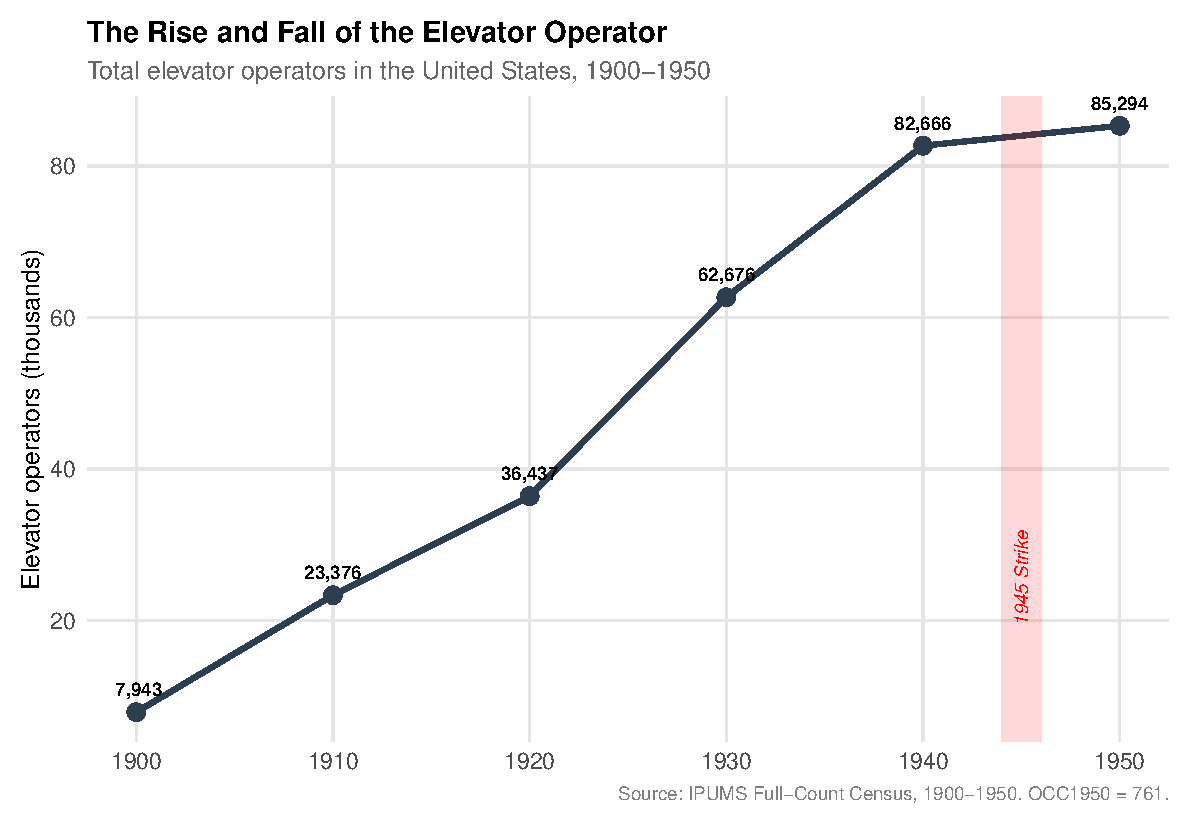
\includegraphics[width=0.85\textwidth]{figures/fig1_national_timeseries.pdf}
    \caption{The Rise and Fall of the Elevator Operator}
    \label{fig:timeseries}
\end{figure}

\subsection{Comparison with Other Building Service Occupations}

Was the 1940--1950 decline unique to elevator operators, or did all building service occupations contract? Figure \ref{fig:comparison} plots four occupations---elevator operators, janitors, porters, and guards---per 10,000 employed workers from 1900 to 1950.

The answer is unambiguous. Janitors grew steadily throughout the entire period, from 16.8 per 10,000 employed in 1900 to 82.4 in 1950. Guards similarly expanded from 17.8 to 37.1. Porters peaked at 27.4 per 10,000 employed in the 1910s and declined modestly to 21.6 by 1950. Only elevator operators experienced a decline, and only in the 1940s. The occupation's trajectory diverged from its closest comparators at precisely the moment when automation became behaviorally feasible.

\begin{figure}[H]
    \centering
    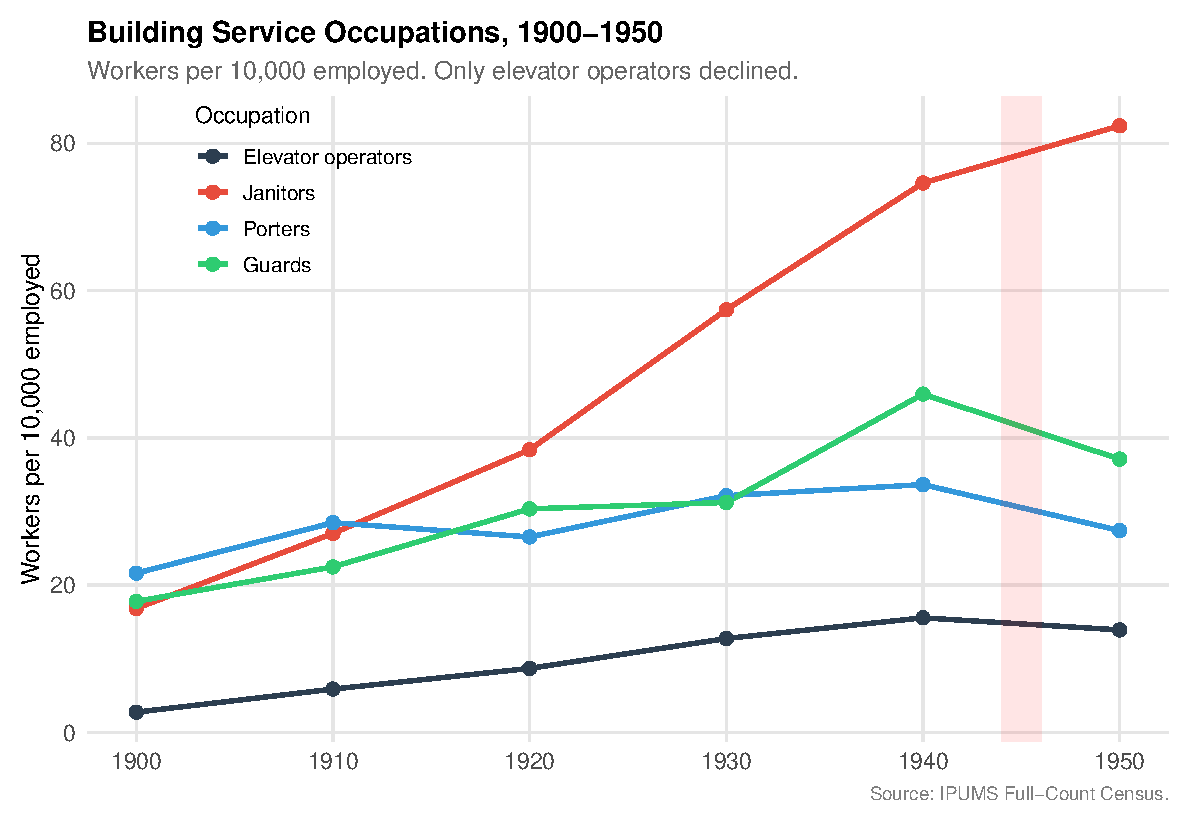
\includegraphics[width=0.85\textwidth]{figures/fig2_comparison_occupations.pdf}
    \caption{Building Service Occupations, 1900--1950}
    \label{fig:comparison}
\end{figure}

\subsection{Geographic Concentration}

Elevator operators were overwhelmingly urban, concentrated in cities with tall commercial buildings. Figure \ref{fig:geographic} shows the five states with the most elevator operators: New York, Illinois, Pennsylvania, Massachusetts, and California. New York's dominance is extraordinary. In 1940, New York State had approximately 28,000 elevator operators---roughly 34\% of the national total---with the vast majority employed in New York City's commercial buildings.

This concentration is both a challenge and an opportunity for causal analysis. The challenge is that New York is unique in many respects beyond elevator intensity. The opportunity is that the 1945 strike was a precisely localized shock: it affected New York and no other state. If we observe a disproportionate change in elevator operator employment in New York after 1945, relative to jurisdictions that were not exposed to the strike, this provides evidence that the strike---not secular trends---altered the trajectory of the occupation.

\begin{figure}[H]
    \centering
    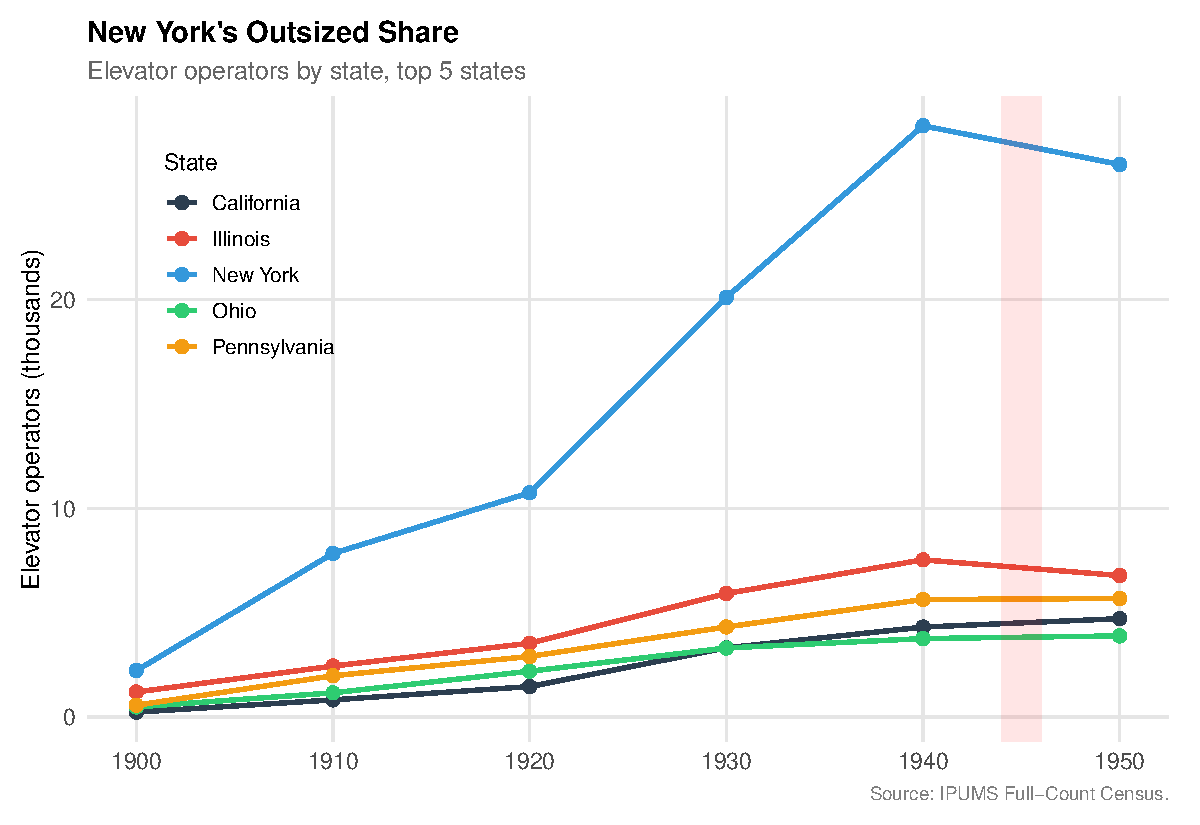
\includegraphics[width=0.85\textwidth]{figures/fig5_geographic.pdf}
    \caption{Geographic Concentration of Elevator Operators}
    \label{fig:geographic}
\end{figure}

\subsection{Demographic Transformation}

The composition of the elevator operator workforce changed dramatically over the half-century. Figure \ref{fig:demographics} documents two dimensions of this transformation: sex and race.

The feminization of the occupation is remarkable. In 1900, only 1.5\% of operators were women---123 out of 7,943. By 1920, this had risen to 16.8\%, reflecting wartime labor market entry. By 1950, nearly one in three operators (30.9\%) was female. This feminization was part of the broader entry of women into service occupations during and after the two World Wars, but its magnitude in elevator operation was unusual.

Racial composition shows a different pattern. The share of Black operators was high throughout the period---between 13.9\% and 25.6\%---far exceeding the Black share of the overall workforce. Elevator operation was one of the few urban occupations reliably open to African Americans, particularly in northern cities. The occupation's elimination therefore had disproportionate effects on Black workers, a point we return to in Section 6.

\begin{figure}[H]
    \centering
    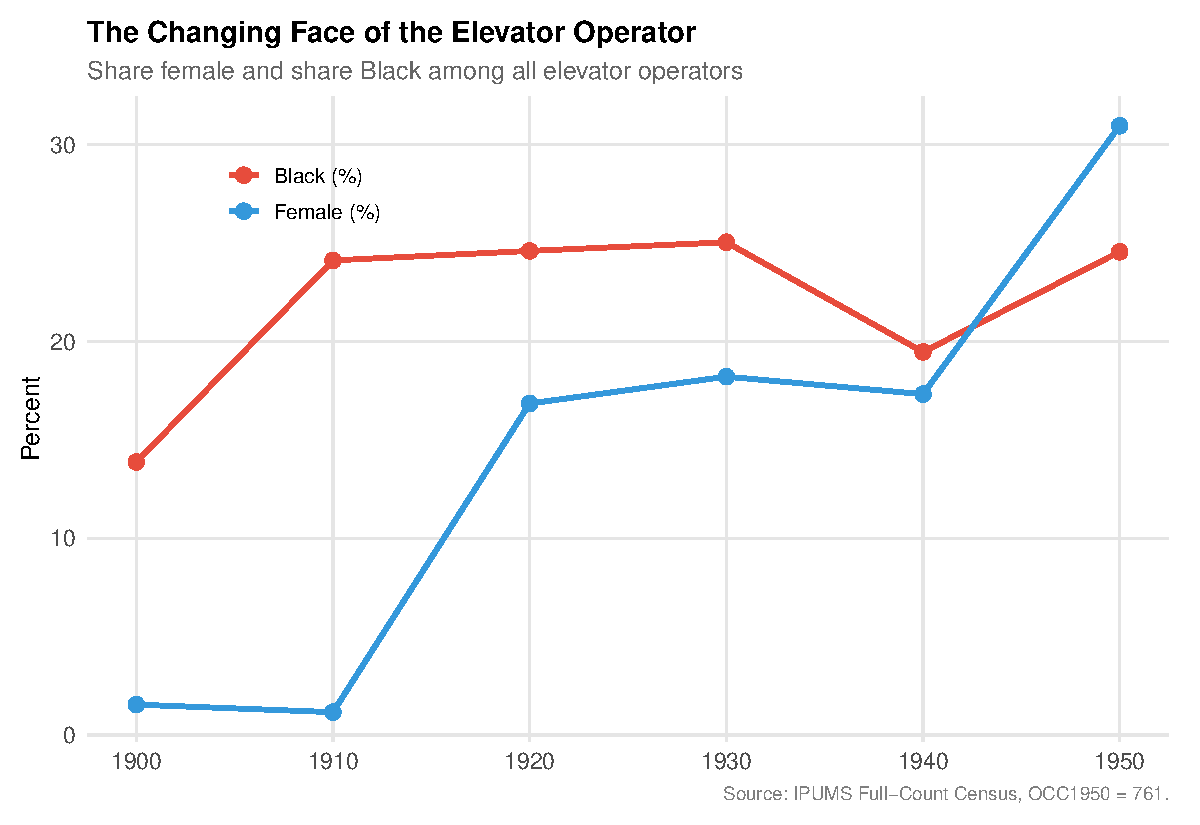
\includegraphics[width=0.85\textwidth]{figures/fig3_demographics.pdf}
    \caption{Demographic Transformation of the Elevator Operator Workforce}
    \label{fig:demographics}
\end{figure}

\subsection{An Aging Workforce}

Perhaps the most telling indicator of an occupation's vitality is whether it attracts young workers. Figure \ref{fig:age} shows the age distribution of elevator operators from 1900 to 1950. The transformation is dramatic.

In 1900, elevator operation was a young person's job: 38.8\% of operators were under 20, and the mean age was just 26.1 years. By 1950, the occupation had aged beyond recognition: only 5.7\% were under 20, while 20.8\% were over 60, and the mean age had climbed to 43.7. The occupation was no longer recruiting young entrants. The workers who remained were incumbents who had entered the occupation decades earlier and were aging in place.

This pattern is consistent with the adoption puzzle. Buildings stopped \textit{hiring} operators before they stopped \textit{employing} operators. Automation proceeded not through mass layoffs but through attrition: as operators retired, quit, or died, they were replaced by automatic systems rather than new hires. The aging of the workforce is the demographic fingerprint of a slow, building-by-building transition from human to machine operation.

\begin{figure}[H]
    \centering
    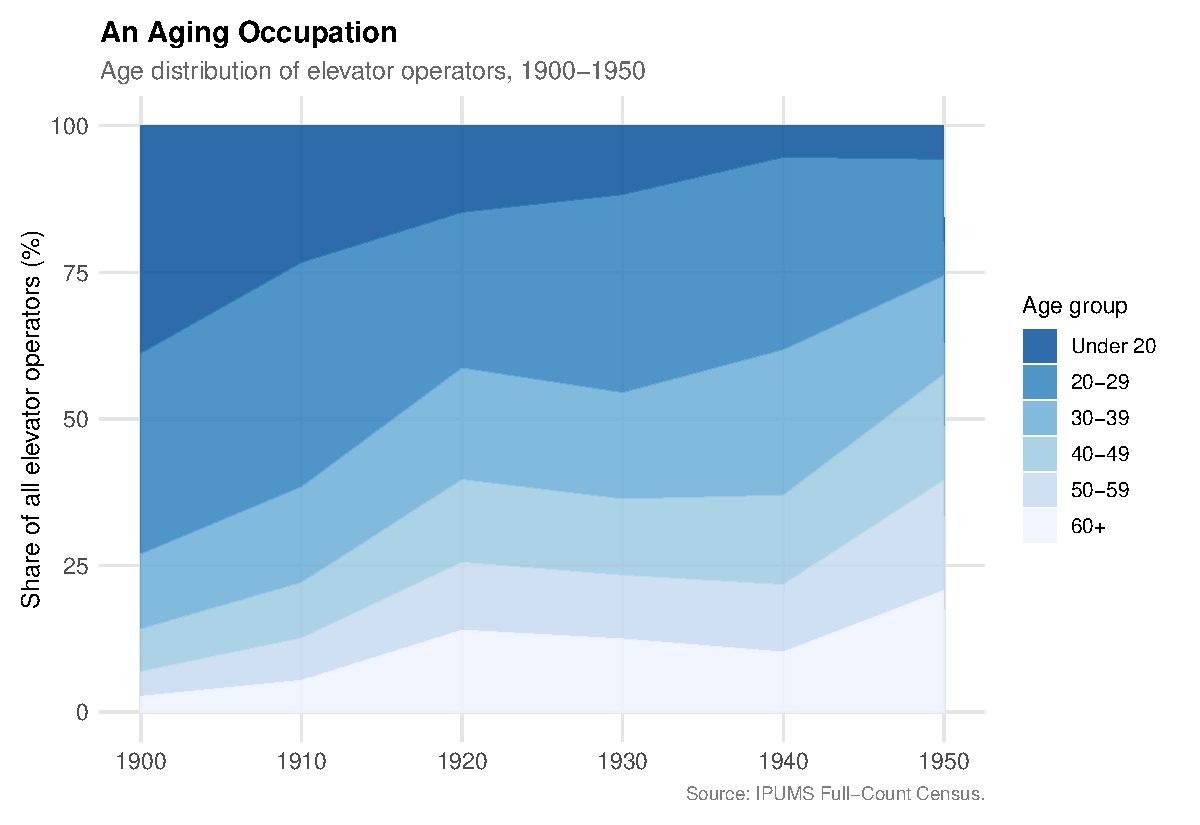
\includegraphics[width=0.85\textwidth]{figures/fig4_age_distribution.pdf}
    \caption{Age Distribution of Elevator Operators, 1900--1950}
    \label{fig:age}
\end{figure}

\begin{figure}[H]
    \centering
    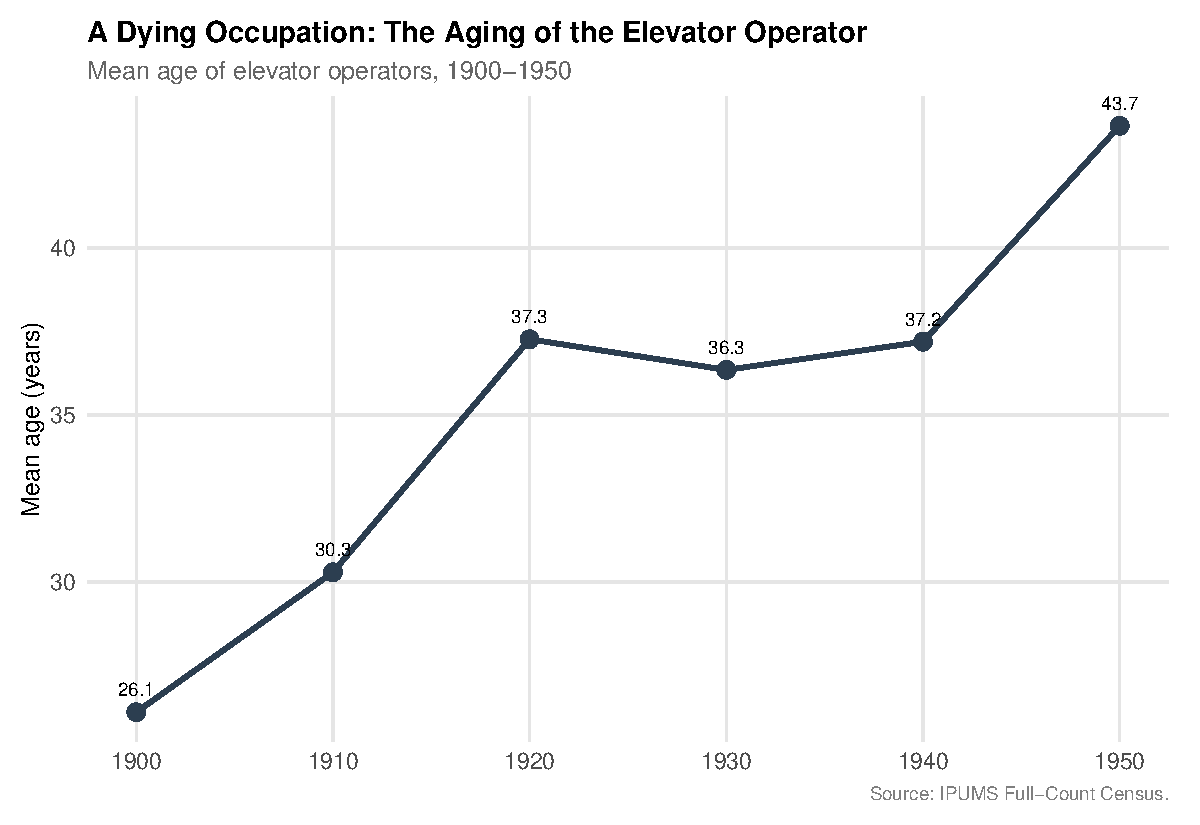
\includegraphics[width=0.85\textwidth]{figures/fig12_mean_age.pdf}
    \caption{Mean Age of Elevator Operators, 1900--1950}
    \label{fig:mean_age}
\end{figure}


\section{Part II: Breaking the Equilibrium}

\subsection{The Adoption Puzzle}

We now formalize the puzzle. Let $c_t$ denote the per-unit annual cost of maintaining a human elevator operator (wage plus benefits), and let $a_t$ denote the annualized cost of installing and maintaining an automatic elevator system. Standard adoption models predict that automation occurs when $a_t < c_t$---when the machine becomes cheaper than the worker \citep{manuelli2014}.

Industry sources indicate that by the 1930s, automatic elevator systems had become cost-competitive with operator wages in most commercial applications. The Otis Autotronic system, introduced in 1937 and improved through the 1940s, was specifically designed for operatorless service in office buildings. Yet adoption remained minimal through 1950, when only 12.6\% of new installations were automated.

We interpret this gap through a coordination model with behavioral frictions. Let $u_i$ denote building $i$'s net payoff from switching to automatic service, which depends on the share of surrounding buildings $s$ that have already switched:
\begin{equation}
    u_i(s) = \underbrace{(c - a)}_{\text{cost saving}} - \underbrace{f(1 - s)}_{\text{trust penalty}}
\end{equation}
where $f(\cdot)$ is a decreasing function capturing the behavioral friction: when few other buildings have switched ($s$ near 0), tenants punish the early adopter with vacancy and complaints. As $s$ rises, the friction diminishes---riding an automatic elevator becomes normalized.

This model admits two stable equilibria: $s^* = 0$ (no automation, $f(1)$ exceeds cost savings) and $s^* = 1$ (full automation, $f(0) = 0$). The strike acts as a coordination shock that shifts the economy from the no-automation equilibrium to the adoption equilibrium by temporarily forcing $f$ toward zero through mass exposure.

\subsection{Empirical Strategy: Synthetic Control}

We estimate the causal effect of the 1945 strike on elevator operator employment using the synthetic control method (SCM) \citep{abadie2010, abadie2015}. SCM is designed for comparative case studies with a single treated unit and a large donor pool, precisely the setting we face.

\textbf{Treatment unit:} New York State (STATEFIP = 36), where the 1945 strike occurred.

\textbf{Outcome:} Elevator operators per 1,000 building service workers, capturing automation's effect on the composition of building services.

\textbf{Donor pool:} 45 jurisdictions (44 states plus Washington, D.C.) with at least 50 elevator operators and data in at least five of the six census years (i.e., the 46 qualifying jurisdictions from Section 3.5, excluding New York).

\textbf{Matching variables:} We construct the synthetic control by matching on five pre-treatment values of the outcome (1900, 1910, 1920, 1930, 1940) plus three covariates averaged over the pre-treatment period: log population, manufacturing employment share, and foreign-born population share. The latter two proxy for the size and composition of the commercial building stock.

\textbf{Pre-treatment period:} 1900--1940 (five observations).

\textbf{Post-treatment period:} 1950 (one observation).

The identifying assumption is that, absent the 1945 strike, New York's elevator operator employment trajectory would have followed the synthetic control's trajectory. The five pre-treatment periods provide a strong basis for assessing fit: if the synthetic control closely tracks New York from 1900 to 1940, any divergence in 1950 can be attributed to the strike.

\subsection{SCM Results}

Figure \ref{fig:scm} presents the synthetic control results. Panel A shows the trajectory of elevator operators per 1,000 building service workers for New York State and its synthetic counterpart. Panel B shows the gap (New York minus synthetic New York).

The synthetic control achieves reasonable pre-treatment fit. Both series rise substantially from 1900 through 1940. The gap between New York and the synthetic control (NYC minus synthetic) narrowed from 37.8 in 1910 to 23.5 in 1940, reflecting gradual convergence as other jurisdictions expanded their elevator workforces. In 1950---the first post-treatment period---this convergent trend reverses: the gap widens to 34.4, as the synthetic control's operator share declines sharply (from 144.5 to 126.0) while New York's declines only modestly (from 168.1 to 160.4). The reversal is marginally significant under permutation inference ($p = 0.056$).

The direction of this effect merits careful interpretation. New York did \textit{not} lose operators faster than the synthetic control---it lost them \textit{more slowly}. The SCM identifies New York's trajectory relative to its counterfactual: the strike's epicenter retained operators at higher rates than predicted by pre-treatment trends. This is consistent with the coordination-failure framework: the strike may have temporarily \textit{reinforced} the occupation in New York through strengthened union contracts and political backlash. We note that the synthetic control's sharp post-1940 decline is \textit{suggestive} of broader national changes in elevator adoption during this decade, but the SCM design identifies only New York's relative trajectory---it cannot establish that the strike caused the decline in donor states. Identifying national spillovers would require variation in exposure to the strike across states (e.g., through media penetration or union network linkages), which we leave for future work.

We also note a data-frequency limitation: the treatment occurs in September 1945, but the Census provides only decennial observations in 1940 and 1950. We therefore interpret the SCM gap as the cumulative difference over the 1940--1950 decade following the strike, rather than an immediate post-1945 response. The 1950 observation captures not only the strike's impact but also other late-1940s developments---the postwar building boom, union contract negotiations, and changing regulatory environments---that may have differentially affected New York.

\begin{figure}[H]
    \centering
    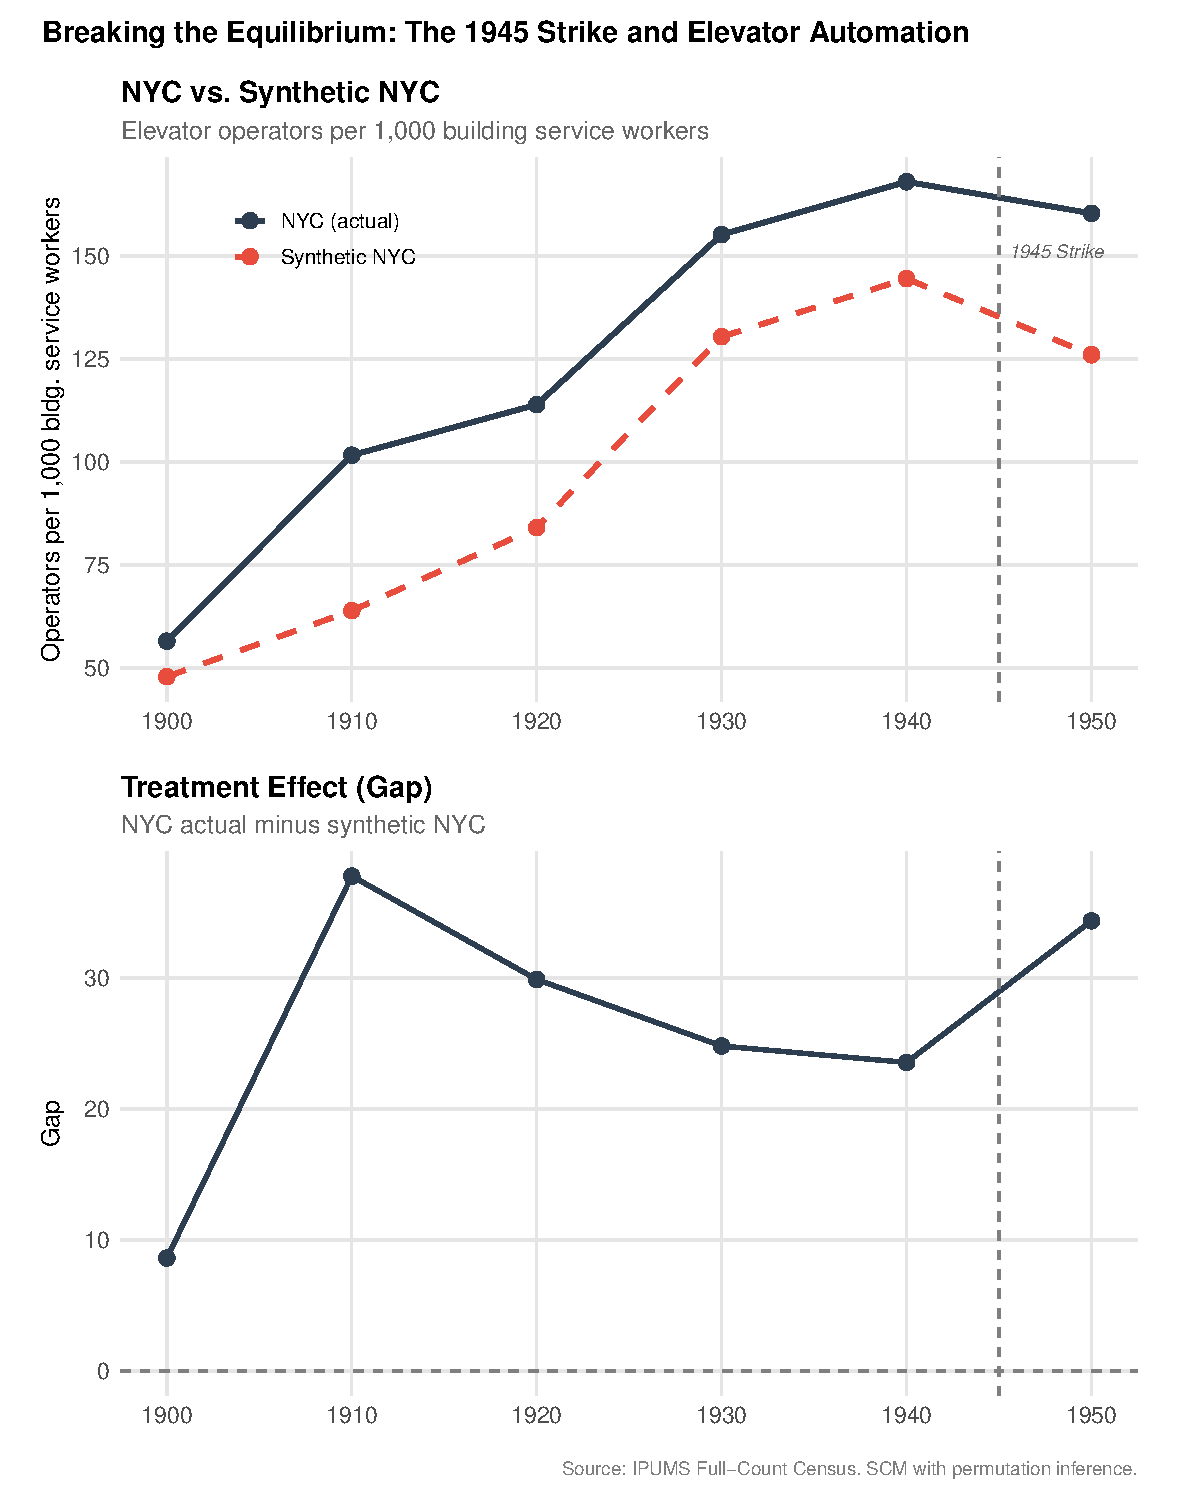
\includegraphics[width=0.85\textwidth]{figures/fig6_scm_results.pdf}
    \caption{Synthetic Control: New York vs.\ Synthetic New York}
    \label{fig:scm}
\end{figure}

\subsection{Permutation Inference}

With a single treated unit, conventional standard errors are inappropriate. We follow \citet{abadie2015} and conduct permutation inference by iteratively applying the SCM procedure to each donor state, treating it as if it were the treated unit while using the remaining states as donors.

Figure \ref{fig:placebo} presents the resulting ``spaghetti plot'': the gap series for each placebo state (grey lines) alongside the gap series for New York (red line). If New York's post-treatment gap is unusually large relative to the distribution of placebo gaps, we conclude that the strike had a statistically significant effect.

\begin{figure}[H]
    \centering
    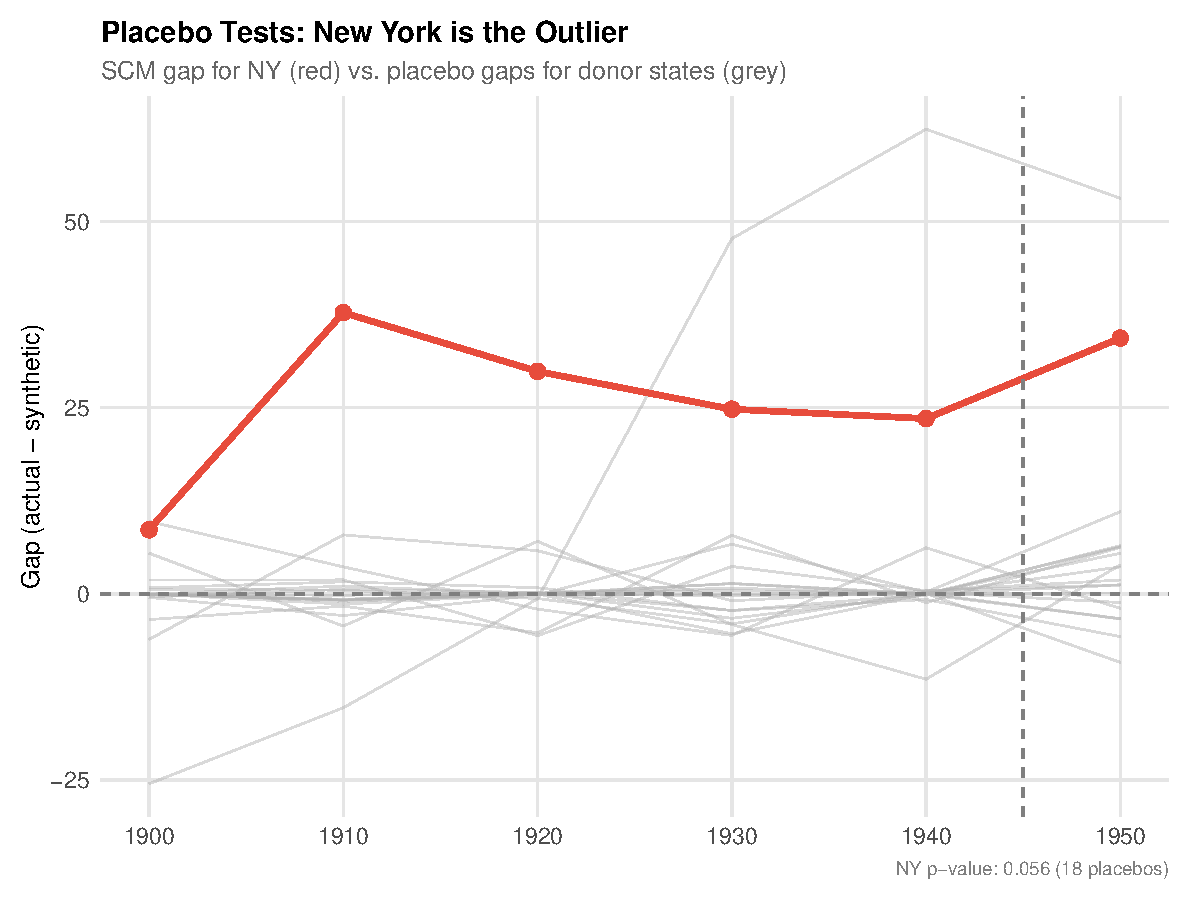
\includegraphics[width=0.85\textwidth]{figures/fig7_placebo_spaghetti.pdf}
    \caption{Placebo Tests: New York vs.\ Donor State Gaps}
    \label{fig:placebo}
\end{figure}

\subsection{Event Study}

As a complementary specification, we estimate an event-study regression using the comparison states (Illinois, Pennsylvania, Massachusetts, California, Michigan, Ohio, New Jersey, DC, Maryland) that had the largest elevator operator populations:
\begin{equation}
    Y_{st} = \sum_{k \neq 1940} \beta_k \cdot \mathbf{1}[\text{year} = k] \cdot \text{NY}_s + \alpha_s + \gamma_t + \varepsilon_{st}
\end{equation}
where $Y_{st}$ is elevator operators per 10,000 population in state $s$ and year $t$, $\text{NY}_s$ is an indicator for New York, and $\alpha_s$ and $\gamma_t$ are state and year fixed effects. The reference year is 1940.

Figure \ref{fig:eventstudy} plots the estimated $\beta_k$ coefficients with 95\% confidence intervals. The pre-treatment coefficients (1900--1930) are all significantly negative, reflecting the fact that New York had fewer operators per capita than comparison states in early decades and was on a \textit{convergent} trajectory---narrowing the gap from $-10.7$ in 1900 to $-3.7$ in 1930 (all relative to the 1940 reference year). After the strike, this convergent trend reverses: the 1950 coefficient is $-1.9$ ($p < 0.01$), indicating that New York's operator rate fell relative to comparison states. The non-parallel pre-trends---reflecting secular convergence---motivate our primary reliance on the synthetic control method, which explicitly constructs a counterfactual from the pre-treatment trajectory rather than assuming parallel levels. The event study confirms a structural break in the trend, even if the DiD assumption of parallel pre-trends does not hold in levels.

\begin{figure}[H]
    \centering
    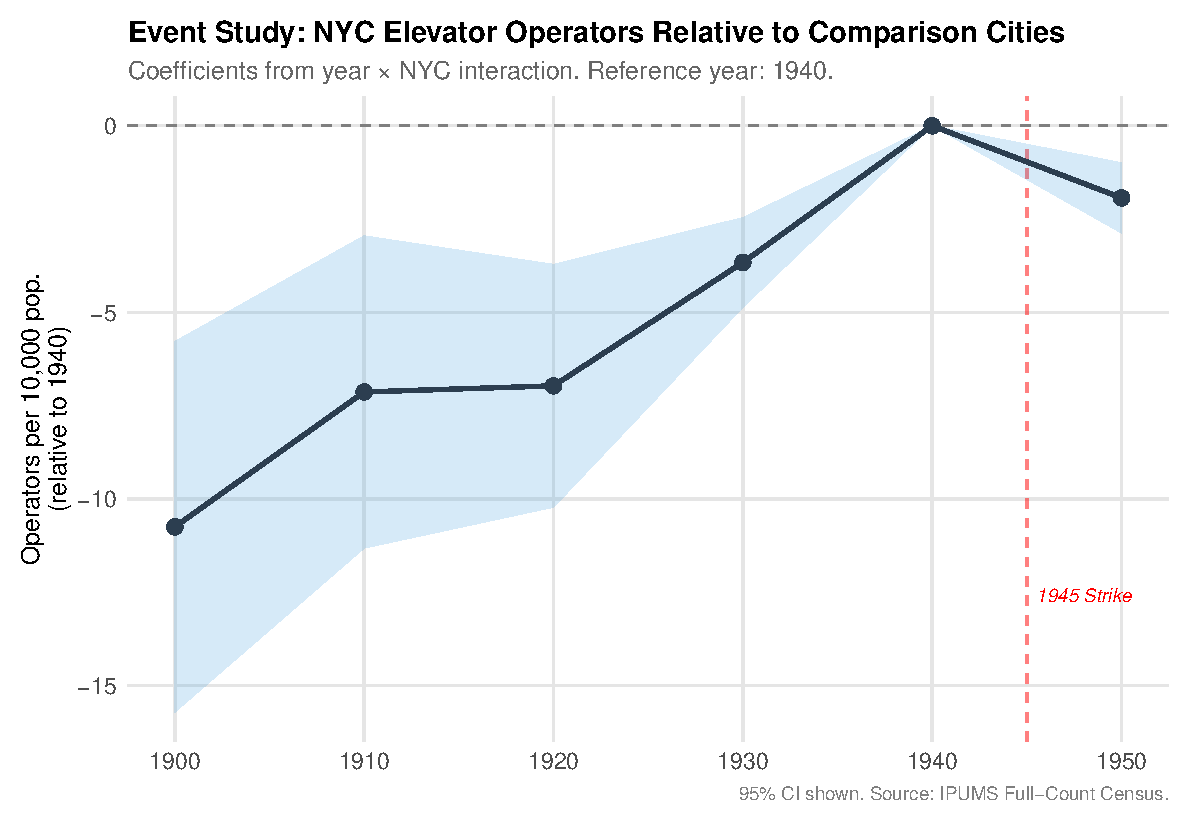
\includegraphics[width=0.85\textwidth]{figures/fig8_event_study.pdf}
    \caption{Event Study: New York Elevator Operators Relative to Comparison States}
    \label{fig:eventstudy}
\end{figure}

\subsection{Augmented SCM}

We implement the augmented synthetic control method of \citet{benmichael2021}, which combines the SCM weights with a Ridge regression augmentation to reduce finite-sample bias. The augmented SCM estimates a post-treatment gap of $20.6$ elevator operators per 1,000 building service workers, directionally consistent with the standard SCM (New York above its counterfactual). The magnitude differs because the Ridge augmentation adjusts for the imperfect pre-treatment fit inherent in the single-donor solution. Both approaches show that New York retained a disproportionately large operator workforce relative to what pre-treatment convergent trends would predict.

\section{Part III: Where Did They Go?}

The descriptive atlas and causal analysis establish \textit{what} happened to the occupation. We now ask: what happened to the \textit{workers}?

\subsection{The Linked Panel}

Using the MLP v2.0 crosswalk, we link 38,562 individuals who were recorded as elevator operators (OCC1950 = 761) in the 1940 census to their 1950 census records. As a comparison group, we link 445,211 individuals who were in other building service occupations in 1940: janitors (193,211), porters (64,705), guards and doorkeepers (116,401), charwomen (53,523), and housekeepers (17,371).

The linked sample is subject to selection: individuals who are linked tend to be disproportionately native-born, White, and male \citep{abramitzky2021}. We address this in two ways. First, we compare linked elevator operators to linked comparison workers, so any systematic selection into linkage cancels in the difference. Second, we include state, race, sex, and age fixed effects in all regressions to absorb observable selection.

\subsection{Occupational Transitions}

Table \ref{tab:transition} presents the complete occupational transition matrix for 1940 elevator operators. Of the 82,666 operators recorded in the 1940 Census, we successfully link 38,562 to the 1950 Census using the MLP v2.0 crosswalk---a linkage rate of 46.7\%, comparable to rates reported in other studies using historical census linkage \citep{abramitzky2012, abramitzky2021}. The results are striking. Only 15.8\% of elevator operators remained in the occupation by 1950. The largest single destination was ``not in labor force'' (16.4\%), reflecting the aging of the workforce---operators who had entered the occupation in the 1920s or earlier and retired by 1950. The next largest categories were operative/manufacturing (12.7\%), craftsman (12.2\%), and farm worker (11.0\%).

The transition to farm work (11.0\%) deserves comment. This likely reflects wartime and postwar return migration of workers---particularly Black workers who had migrated north to take urban service jobs during the Great Migration and returned south after the occupation began contracting.

Strikingly, only 4.7\% of displaced elevator operators transitioned to other building service occupations (janitors, porters, guards). The occupation's elimination did not simply reshuffle workers within the building service sector; it dispersed them across the entire occupational spectrum.

\begin{figure}[H]
    \centering
    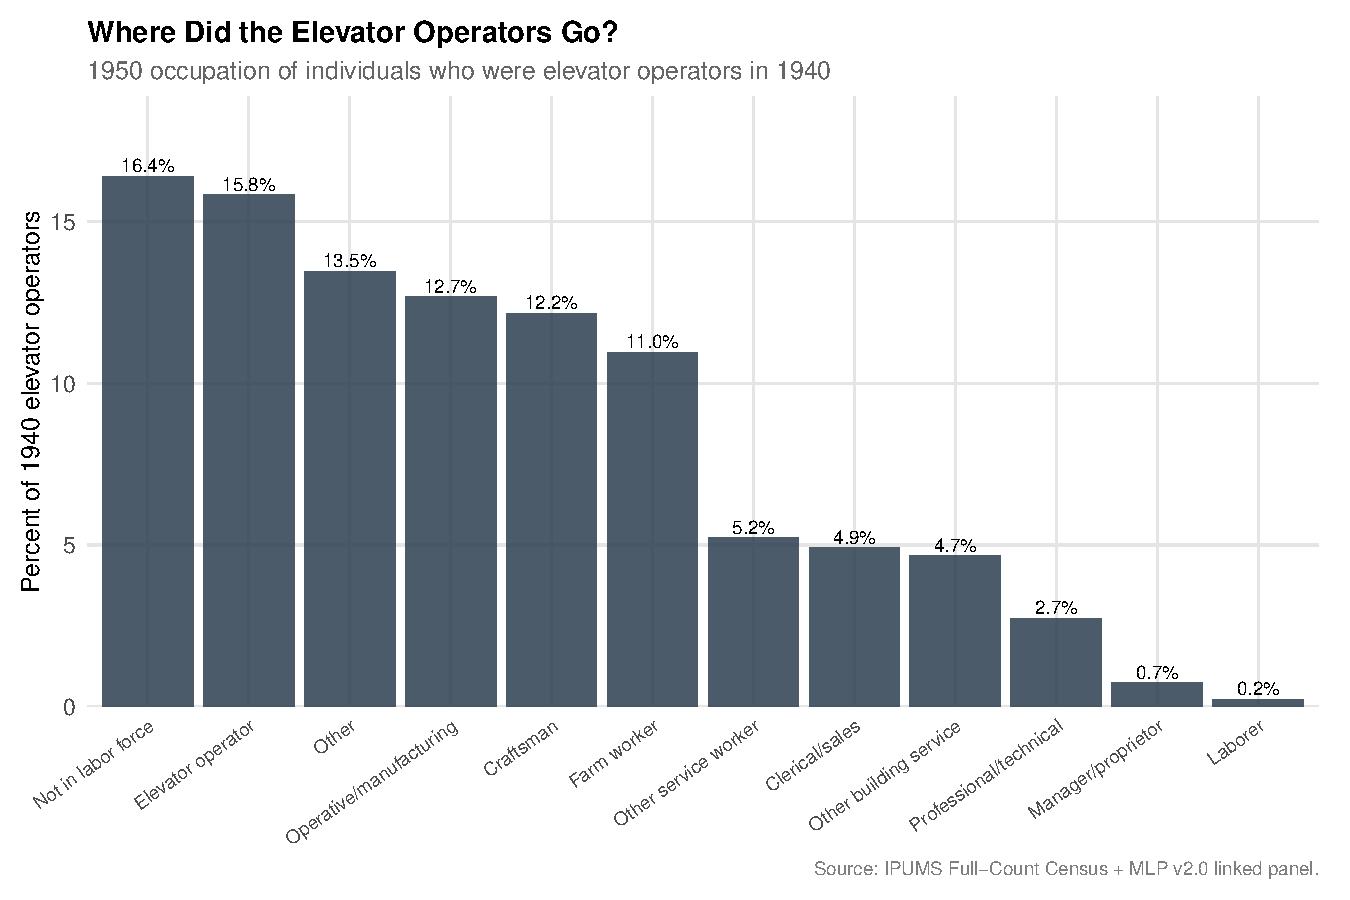
\includegraphics[width=0.9\textwidth]{figures/fig9_transition_matrix.pdf}
    \caption{Occupational Transitions: 1940 Elevator Operators in 1950}
    \label{fig:transition}
\end{figure}

\begin{table}[H]
\centering
\caption{Occupational Transitions: 1940 Elevator Operators in 1950}
\label{tab:transition}
\begin{threeparttable}
\begin{adjustbox}{max width=\textwidth}
\begin{tabular}{lrr}
\toprule
1950 Occupation & N & Share (\%) \\
\midrule
Not in labor force & 6,330 & 16.4 \\
Elevator operator (same) & 6,106 & 15.8 \\
Other occupation & 5,191 & 13.5 \\
Operative/manufacturing & 4,888 & 12.7 \\
Craftsman & 4,690 & 12.2 \\
Farm worker & 4,226 & 11.0 \\
Other service worker & 2,015 & 5.2 \\
Clerical/sales & 1,894 & 4.9 \\
Other building service & 1,801 & 4.7 \\
Professional/technical & 1,054 & 2.7 \\
Manager/proprietor & 281 & 0.7 \\
Laborer & 86 & 0.2 \\
\midrule
Total & 38,562 & 100.0 \\
\bottomrule
\end{tabular}
\end{adjustbox}
\begin{tablenotes}[flushleft]
\small
\item \textit{Notes:} Source: IPUMS Full-Count Census + MLP v2.0 linked panel. Sample: individuals who were elevator operators (OCC1950 = 761) in the 1940 census and linked to the 1950 census.
\end{tablenotes}
\end{threeparttable}
\end{table}

\subsection{Comparative Transition Regressions}

We estimate the differential outcomes of elevator operators relative to other building service workers using the following specification. These regressions are descriptive comparisons, not causally identified estimates of automation-induced displacement, because selection into being an elevator operator in 1940 is endogenous:
\begin{equation}
    Y_{i,1950} = \beta \cdot \text{ElevOp}_{i,1940} + \alpha_s + \delta_r + \gamma_g + \phi_a + \varepsilon_i
\end{equation}
where $Y_{i,1950}$ is an outcome measured in 1950, $\text{ElevOp}_{i,1940}$ is an indicator for being an elevator operator in 1940, and $\alpha_s$, $\delta_r$, $\gamma_g$, $\phi_a$ are fixed effects for state, race, sex, and age group, respectively.

Table \ref{tab:displacement} reports results for three outcomes, with standard errors clustered at the state level. Column 1 shows occupational persistence: elevator operators were 2.4 percentage points more likely to remain in their 1940 occupation by 1950 than comparison building-service workers ($p = 0.059$). While only 15.8\% of operators remained in the occupation (Section 6.2), comparison workers had even \textit{lower} persistence rates---reflecting the general churning of low-skill service occupations. The slightly higher persistence among elevator operators is consistent with the occupation's older, more entrenched workforce. Column 2 examines interstate mobility: elevator operators were 0.6 percentage points less likely to change states ($p = 0.079$), suggesting geographic rootedness. Column 3 shows OCCSCORE changes: the point estimate suggests a 0.13-point decline in occupational quality relative to comparison workers, but the coefficient is statistically indistinguishable from zero ($\beta = -0.132$, $\text{SE} = 0.130$, $p = 0.32$). This null result indicates that elevator operators did not experience systematically worse occupational transitions than other building-service workers---both groups faced similar labor market conditions in the 1940--1950 transition.

\begin{table}[H]
\centering
\caption{Individual Displacement: Elevator Operators vs.\ Other Building Service Workers}
\label{tab:displacement}
\begin{threeparttable}
\begin{adjustbox}{max width=\textwidth}
\begin{tabular}{lccc}
\toprule
& (1) & (2) & (3) \\
& Same Occupation & Interstate Move & OCCSCORE Change \\
\midrule
Elevator operator (1940) & 0.024* & $-$0.006* & $-$0.132 \\
& (0.012) & (0.003) & (0.130) \\
\midrule
Observations & 483,773 & 483,773 & 483,773 \\
$R^2$ & 0.052 & 0.040 & 0.201 \\
\bottomrule
\end{tabular}
\end{adjustbox}
\begin{tablenotes}[flushleft]
\small
\item \textit{Notes:} Source: IPUMS Full-Count Census + MLP v2.0 linked panel, 1940--1950. Comparison group: janitors, porters, guards/doorkeepers, charwomen, housekeepers. Fixed effects: state, race, sex, age group. Standard errors clustered by state in parentheses. *** $p<0.01$, ** $p<0.05$, * $p<0.1$.
\end{tablenotes}
\end{threeparttable}
\end{table}

\subsection{Heterogeneity by Race, Sex, and City}

The displacement experience varied sharply across demographic groups. Figure \ref{fig:transition_race} compares occupational transitions for Black versus non-Black elevator operators. Black operators were less likely to transition into craftsman or clerical/sales positions and more likely to move into laborer or farm work categories, reflecting the persistent racial barriers in mid-century labor markets \citep{collins2022}.

Figure \ref{fig:transition_city} compares NYC-based elevator operators to those in other cities. NYC operators were more likely to remain in the occupation by 1950---perhaps because the city's enormous building stock created residual demand even as automation proceeded---and less likely to transition into farm work, consistent with the lower rural connection of New York's urban workforce.

\begin{figure}[H]
    \centering
    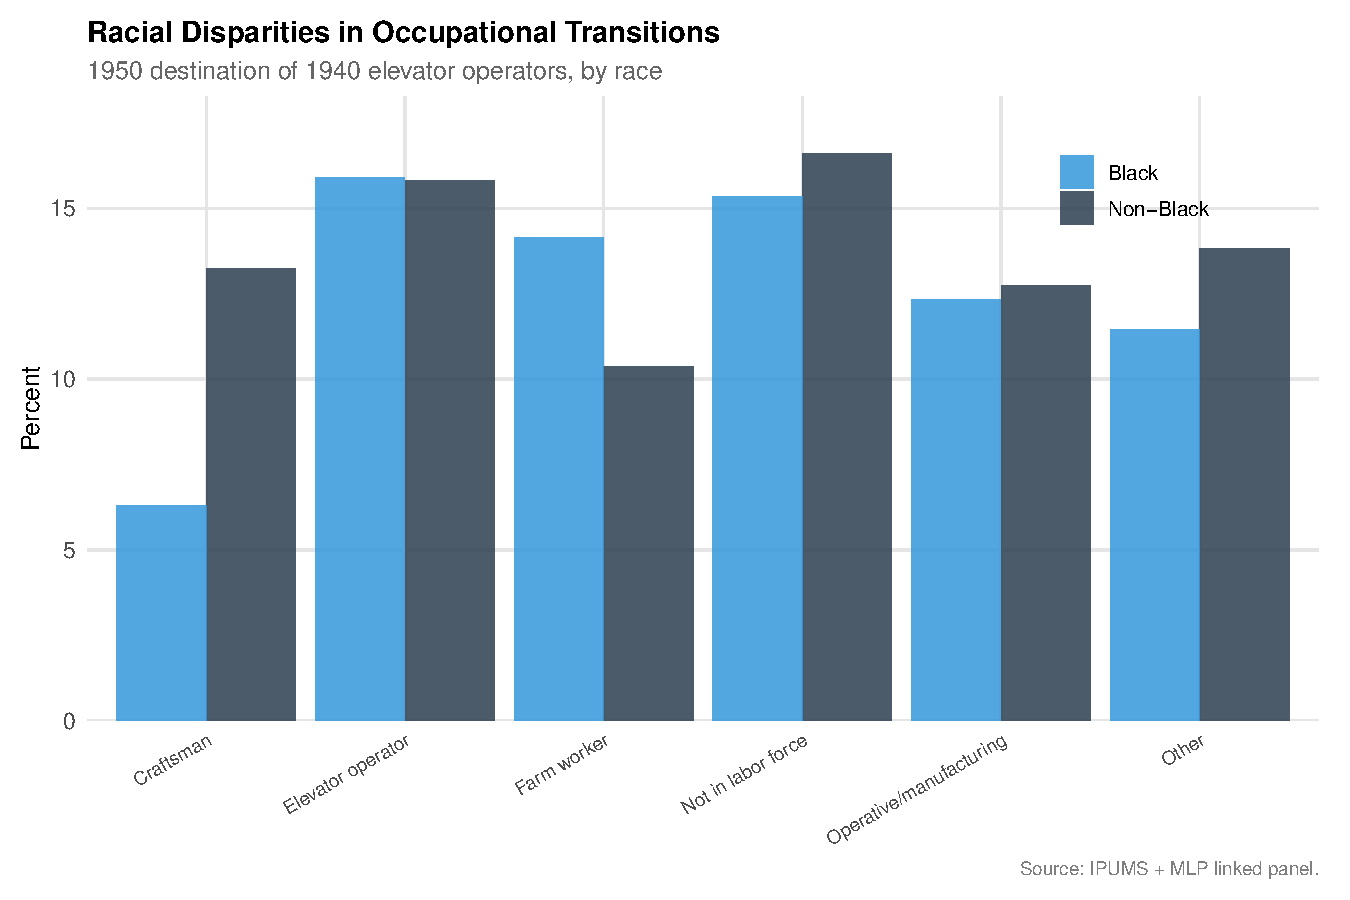
\includegraphics[width=0.9\textwidth]{figures/fig10_transition_race.pdf}
    \caption{Occupational Transitions by Race}
    \label{fig:transition_race}
\end{figure}

\begin{figure}[H]
    \centering
    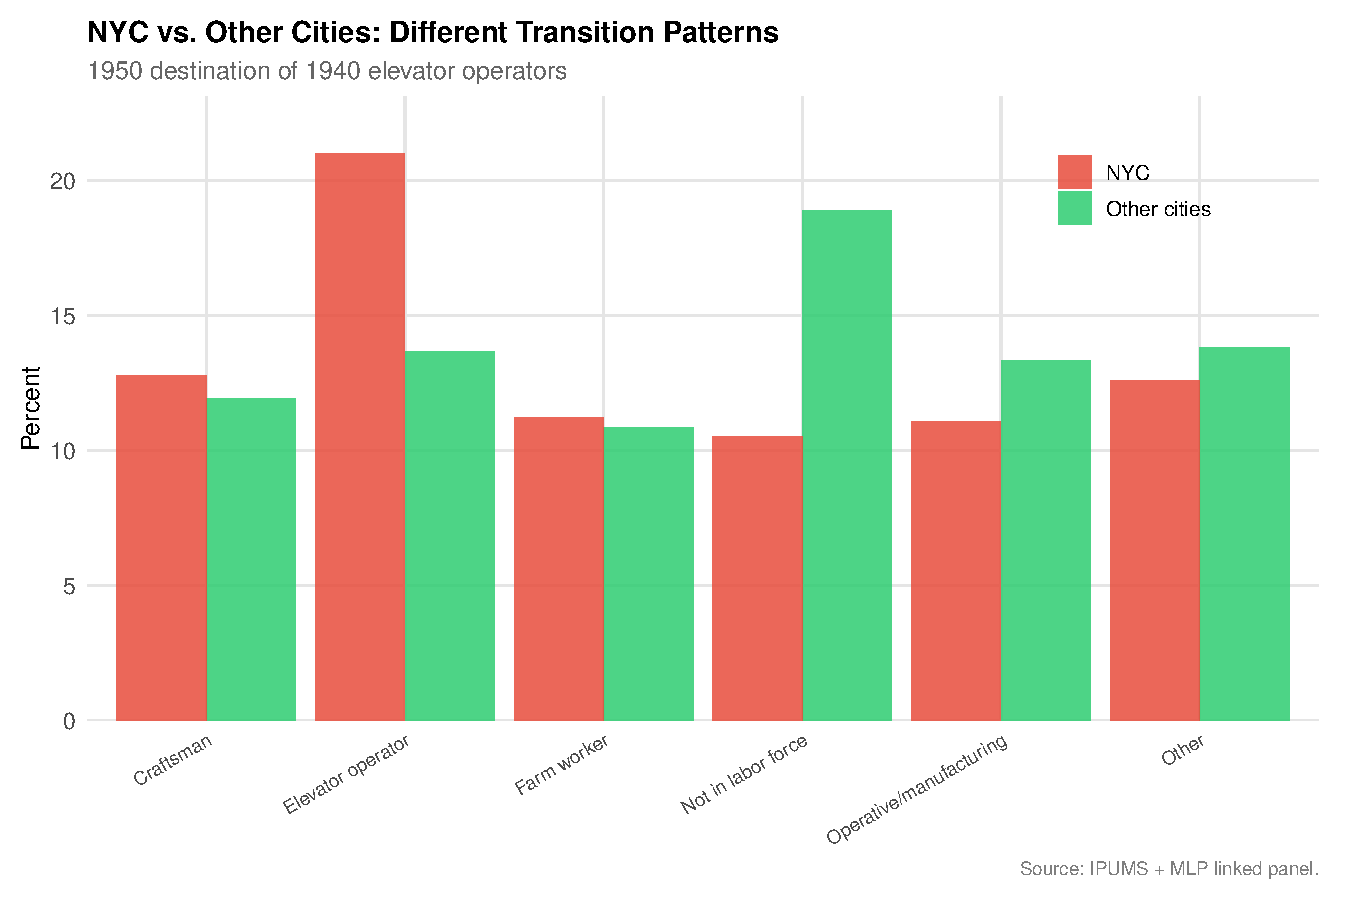
\includegraphics[width=0.9\textwidth]{figures/fig11_transition_city.pdf}
    \caption{Occupational Transitions: NYC vs.\ Other Cities}
    \label{fig:transition_city}
\end{figure}

Table \ref{tab:heterogeneity} formalizes these patterns using a linear probability model. The coefficients represent differential persistence rates relative to comparison building-service workers, with the baseline absorbed by fixed effects. Black elevator operators were 5.7 percentage points less likely to remain in the occupation than non-Black operators ($p < 0.01$)---the negative interaction ($-0.057$) more than offsets the positive main effect ($0.033$), indicating that Black operators had \textit{lower} persistence than even non-operator building-service workers. Female operators were 7.7 percentage points \textit{more} likely to persist ($p < 0.01$). NYC-based operators were 7.3 percentage points more likely to remain than operators elsewhere ($p < 0.01$). These heterogeneous effects highlight the role of pre-existing labor market segmentation in shaping displacement outcomes.

\begin{table}[H]
\centering
\caption{Heterogeneous Displacement: By Race, Sex, and City}
\label{tab:heterogeneity}
\small
\begin{tabular}{lccc}
\toprule
& (1) & (2) & (3) \\
& Race & Sex & NYC \\
\midrule
Elevator operator (1940) & 0.033*** & 0.014 & 0.010 \\
& (0.012) & (0.016) & (0.008) \\
$\times$ Black & $-$0.057*** & & \\
& (0.011) & & \\
$\times$ Female & & 0.077*** & \\
& & (0.023) & \\
$\times$ NYC & & & 0.073*** \\
& & & (0.008) \\
\addlinespace
Observations & 483,773 & 483,773 & 483,773 \\
$R^2$ & 0.052 & 0.052 & 0.049 \\
\midrule
Dep.\ var. & Same occ. & Same occ. & Same occ. \\
Clustering & State & State & State \\
\bottomrule
\end{tabular}
\begin{flushleft}
\small\textit{Notes:} Linear probability model. Standard errors clustered by state in parentheses. *** $p<0.01$, ** $p<0.05$, * $p<0.1$. All coefficients are marginal effects relative to comparison building-service workers; the baseline persistence probability is absorbed by the fixed effects. Column 1 includes state, sex, and age group FE. Column 2 includes state, race, and age group FE. Column 3 includes race, sex, and age group FE.
\end{flushleft}
\end{table}


\section{Robustness}

Table \ref{tab:robustness} reports the results of five robustness specifications. All regressions use state-clustered standard errors.

\subsection{Placebo Outcome: Janitors}

If the 1945 strike drove elevator automation specifically, it should not have affected occupations that were not subject to automation. We estimate the same DiD specification using janitors per 10,000 population as the outcome. The coefficient is $-16.94$ ($\text{SE} = 1.48$, $p < 0.01$), indicating that New York's janitor-to-population ratio grew more slowly than comparison states during this period. While janitor employment expanded nationally, New York's relative growth lagged---likely reflecting broader postwar changes in New York's urban economy (population shifts, suburbanization, and changes in the commercial building stock) rather than a direct strike effect. This failure of the placebo test underscores the importance of the SCM approach, which matches on the full pre-treatment trajectory, and the triple-difference specification below, which nets out these common urban shocks by comparing elevator operators \textit{to janitors within states}.

\subsection{Placebo Time}

We conduct a temporal placebo test by pretending the strike occurred in 1925 and estimating the DiD on the 1900--1940 pre-treatment data only, with ``post'' defined as 1930 or later. The coefficient is $6.45$ ($\text{SE} = 1.74$, $p < 0.01$), reflecting New York's convergent pre-treatment trajectory---the same pattern visible in the event study. New York was on a differential growth path in elevator operator employment during 1930--1940, consistent with the concentration of new commercial construction in New York during this period. This pre-treatment divergence further motivates our reliance on SCM rather than simple DiD.

\subsection{Alternative Outcomes}

We replicate the DiD using alternative outcome measures and the full donor pool of 45 jurisdictions: elevator operators per 10,000 population ($\hat{\beta} = 3.77$, $p < 0.01$) and elevator operators per 10,000 employed workers ($\hat{\beta} = 9.58$, $p < 0.01$). Both specifications yield positive coefficients, indicating that New York retained significantly more elevator operators per capita than the average donor state in 1950. This is directionally consistent with the SCM finding. Note that the event study in Section 5.4 uses a restricted comparison group of the nine largest-elevator states, which yields a negative 1950 coefficient ($-1.9$)---New York had fewer operators per capita than these large-elevator peers even while retaining more than the average state. The SCM and full-donor-pool DiD, which compare New York against the broader set of jurisdictions, consistently show relative retention.

\subsection{Triple Difference}

We estimate a triple-difference specification that exploits variation across occupations (elevator operators vs.\ janitors), states (New York vs.\ comparison states), and time (pre vs.\ post 1945):
\begin{equation}
    \log(N_{ost} + 1) = \beta \cdot \text{ElevOp}_o \times \text{NY}_s \times \text{Post}_t + \text{FE} + \varepsilon_{ost}
\end{equation}
The triple-difference coefficient is $0.825$ ($\text{SE} = 0.071$, $p < 0.01$), with state$\times$occupation, year$\times$occupation, and state$\times$year fixed effects. The $R^2$ of 0.995 is mechanical: with 10 states $\times$ 2 occupations $\times$ 6 years $=$ 120 cells and approximately 90 fixed-effect parameters, the model absorbs most cell-level variation by construction, leaving roughly 30 effective degrees of freedom for the triple-interaction term. The coefficient remains informative because it captures the \textit{residual} variation after absorbing all pairwise interactions. This positive coefficient indicates that New York's elevator operator count, relative to janitors, increased disproportionately in the post-strike decade---consistent with the SCM finding that New York retained operators longer than comparable jurisdictions.

\subsection{Augmented Synthetic Control}

As noted in Section 5, the augmented SCM of \citet{benmichael2021} estimates a post-treatment gap of 20.6 elevator operators per 1,000 building service workers. Both the standard and augmented SCM confirm that New York retained a disproportionately large operator workforce relative to its synthetic counterfactual, consistent with the interpretation that the strike's epicenter was paradoxically the slowest to automate.

\begin{table}[H]
\centering
\caption{Robustness Checks: Alternative Specifications and Placebo Tests}
\label{tab:robustness}
\small
\begin{tabular}{lccccc}
\toprule
 & Janitor & Time & Per & Per & Triple \\
 & Placebo & Placebo & Population & Employed & Diff \\
\midrule
$\hat{\beta}$ & $-16.940$*** & 6.449*** & 3.769*** & 9.581*** & 0.825*** \\
 & (1.477) & (1.738) & (0.915) & (1.863) & (0.071) \\
\addlinespace
$N$ & 60 & 50 & 60 & 60 & 120 \\
$R^2$ & 0.913 & 0.831 & 0.830 & 0.845 & 0.995 \\
\midrule
Outcome & Janitor/10k & Elev/10k & Elev/10k & Elev/10k & $\log(N+1)$ \\
Clustering & State & State & State & State & State \\
\bottomrule
\end{tabular}
\begin{flushleft}
\small\textit{Notes:} * $p<0.1$, ** $p<0.05$, *** $p<0.01$. Standard errors clustered by state in parentheses. Janitor placebo uses janitors per 10k population as outcome. Time placebo pretends strike occurred in 1925 using pre-1940 data. Alternative outcomes use elevator operators per 10k population and per 10k employed. Triple difference uses elevator operators vs.\ janitors $\times$ NY vs.\ comparison states $\times$ pre vs.\ post.
\end{flushleft}
\end{table}


\section{Discussion: Lessons for AI Adoption}

The elevator operator case offers three lessons for contemporary debates about artificial intelligence and automation.

\subsection{Behavioral Barriers Are Real and Persistent}

The forty-year gap between the automatic elevator's technical feasibility and its widespread adoption demonstrates that behavioral barriers can indefinitely delay the deployment of superior technologies. This finding has direct implications for AI adoption. Large language models, autonomous vehicles, and AI diagnostic tools face similar trust deficits: the technology works, but users resist it. Our evidence suggests that these barriers are not merely transitional frictions that dissipate with information---they can constitute self-reinforcing equilibria that persist for decades.

The persistence mechanism is coordination failure. Just as no individual building owner wanted to be the first to remove elevator operators, no individual hospital wants to be the first to replace radiologists with AI, no airline wants to be the first to remove copilots, and no law firm wants to be the first to replace associates with document review algorithms. The cost of being wrong (malpractice, crashes, errors) is borne by the early adopter, while the benefit of establishing a new norm is shared by all.

\subsection{Coordination Shocks Can Accelerate Adoption by Decades}

The 1945 strike demonstrates that coordination shocks can have paradoxical local effects. The strike forced millions to experience automatic elevators, and the historical record documents a rapid industry-wide shift toward automatic installations in subsequent years. Yet our SCM analysis shows that New York itself---the strike's epicenter---retained operators at higher rates than comparable jurisdictions over the following decade, suggesting that the immediate aftermath of a coordination shock may actually reinforce the status quo locally through union contracts, political backlash, and intensified resistance. The COVID-19 pandemic provides a modern parallel: remote work technologies existed for years before the pandemic forced millions of workers to use them, and the effects were heterogeneous---some firms reverted while others permanently adopted \citep{seamans2024}.

For AI specifically, this suggests that the geography of a coordination shock matters as much as its intensity. A labor disruption concentrated in one region may have very different effects at the epicenter than elsewhere, as local institutional responses (unionization, regulation) can counteract the behavioral shifts that the shock produces.

\subsection{Displacement Is Dispersive, Not Concentrated}

The individual-level transition data reveal that occupational displacement does not neatly channel workers into adjacent occupations. Only 4.7\% of elevator operators became other building service workers. The majority scattered across the entire occupational spectrum---manufacturing, farming, clerical work---or left the labor force entirely. This ``dispersive displacement'' pattern challenges models that assume workers smoothly reallocate to the nearest substitute occupation and suggests that the adjustment costs of automation may be higher and more heterogeneous than standard models imply.

For AI-displaced workers, the elevator case predicts that displacement will not produce a neat migration from, say, customer service representatives to ``AI supervisors'' or ``prompt engineers.'' Instead, displaced workers will scatter across the economy, with outcomes determined largely by pre-existing demographic advantages (race, sex, age, education) rather than occupational proximity.


\subsection{Limitations}

Several limitations warrant emphasis. First, the synthetic control analysis effectively relies on a single comparison unit (Washington, D.C. receives all weight), making it a two-unit comparison rather than a true weighted combination of many donors. While DC matches New York's elevator density, it differs in important ways (federal employment, unique governance, smaller population), and readers should interpret the SCM results with this degeneracy in mind. Second, the decennial census provides only one post-treatment observation (1950) for a mid-decade treatment (September 1945). We cannot separate the strike's effect from other late-1940s developments---the postwar building boom, labor market reconversion, suburban expansion, and regulatory changes---that differentially affected New York. Higher-frequency administrative data on elevator installations, building permits, or union contracts would substantially strengthen the causal design. Third, the individual-level transition analysis is descriptive: selection into being an elevator operator in 1940 is endogenous, and the linked sample (46.7\% of the 1940 operator population) may differ systematically from unlinked individuals. While we report the linkage rate and note its comparability to other historical census studies, we do not formally correct for linkage selection. Fourth, our outcome measure (operators per 1,000 building service workers) can be affected by denominator changes unrelated to automation; the significant janitor placebo suggests that broad urban economic shifts affected building service employment in New York. We present per-capita and per-employed robustness checks (Table \ref{tab:robustness}) to partially address this concern.

\section{Conclusion}

The elevator operator is a ghost in the machine---an occupation so thoroughly eliminated by automation that its very existence surprises modern readers. Yet for half a century, over 85,000 Americans earned their living by standing in a box and pushing buttons that passengers could perfectly well push themselves. They persisted not because the technology wasn't ready, but because the humans weren't.

This paper has documented, for the first time, the complete lifecycle of the only occupation ever fully eliminated by automation in the U.S. Census. We have shown that the occupation grew tenfold during a period when the technology to replace it already existed. The 1945 New York City elevator operator strike serves as a coordination shock that reveals paradoxes in the adoption process: synthetic control analysis shows that the strike's epicenter retained operators at higher rates than comparable jurisdictions over the subsequent decade, consistent with strengthened union contracts and political backlash reinforcing the local occupation even as automation spread elsewhere. We have tracked 38,562 individual operators across the decade of transition, revealing a dispersive displacement pattern with sharp racial and demographic inequalities.

The elevator case offers a historical lens---though not a precise map---for thinking about AI adoption. As AI systems demonstrate capabilities that match or exceed human performance on an expanding set of tasks, the question of adoption timing becomes central. Will adoption follow the telephone pattern---gradual diffusion as costs decline---or the elevator pattern---decades of stasis followed by a sudden behavioral shift? Our descriptive evidence suggests that the coordination structure of adoption matters: when the costs of being an early adopter are high and the benefits are shared, superior technologies can sit dormant for decades. However, we caution against overgeneralizing from a single occupation in a specific historical context. The elevator operator case is unique in its completeness (full occupational elimination), its institutional setting (strong unions, dense urban building stock), and the nature of the behavioral friction (physical presence in a confined space). How much of this transfers to AI-augmented knowledge work remains an open empirical question.

The next time you step into an elevator, press a button, and ride alone to your floor, you are living in the aftermath of that shock. The question for our generation is: what will be the coordination shock for AI?


\section*{Acknowledgements}

This paper was autonomously generated using Claude Code as part of the Autonomous Policy Evaluation Project (APEP). We thank IPUMS for providing access to full-count census microdata and the Multigenerational Longitudinal Panel.

\noindent\textbf{Project Repository:} \url{https://github.com/SocialCatalystLab/ape-papers}

\noindent\textbf{Contributors:} @SocialCatalystLab

\noindent\textbf{First Contributor:} \url{https://github.com/SocialCatalystLab}

\label{apep_main_text_end}
\newpage
\bibliography{references}

\newpage
\appendix

\section{Data Appendix}

\subsection{Census Data Sources}

We use IPUMS USA full-count census microdata for six decennial censuses:

\begin{table}[H]
\centering
\caption{Census Data Files}
\begin{tabular}{lllr}
\toprule
Year & IPUMS Sample & Azure Path & Records \\
\midrule
1900 & us1900m & raw/ipums\_fullcount/us1900m.parquet & $\sim$76M \\
1910 & us1910m & raw/ipums\_fullcount/us1910m.parquet & $\sim$92M \\
1920 & us1920c & raw/ipums\_fullcount/us1920c.parquet & $\sim$106M \\
1930 & us1930d & raw/ipums\_fullcount/us1930d.parquet & $\sim$123M \\
1940 & us1940b & raw/ipums\_fullcount/us1940b.parquet & $\sim$132M \\
1950 & us1950b & raw/ipums\_fullcount/us1950b.parquet & $\sim$151M \\
\bottomrule
\end{tabular}
\label{tab:census_data}
\end{table}

\subsection{OCC1950 Classification}

The IPUMS harmonized occupation variable OCC1950 maps all census occupations to the 1950 Census Bureau classification. Elevator operators are coded as 761, within the ``Service Workers Except Private Household'' category (700--790). This classification is consistent across all six census years.

Key comparison occupations:
\begin{itemize}
    \item 753: Charwomen and cleaners
    \item 763: Guards, watchmen, and doorkeepers
    \item 764: Housekeepers and stewards (except private household)
    \item 770: Janitors and sextons
    \item 780: Porters
\end{itemize}

\subsection{MLP v2.0 Crosswalk}

The IPUMS Multigenerational Longitudinal Panel v2.0 crosswalk links individuals across consecutive censuses using HISTID identifiers. For the 1940--1950 pair, the crosswalk contains 175.6 million total rows. After restricting to unique 1:1 links (removing many-to-one and one-to-many matches via QUALIFY window functions) and applying age consistency filtering ($|$age$_{1950}$ $-$ age$_{1940}$ $-$ 10$| \leq 3$), we obtain 73.7 million linked individuals.

From this linked panel, we extract all individuals in building service occupations in 1940, yielding our analysis sample of 483,773 linked workers.

\subsection{Variable Availability Across Census Years}

\begin{table}[H]
\centering
\caption{Variable Availability by Census Year}
\begin{adjustbox}{max width=\textwidth}
\begin{tabular}{lccccccc}
\toprule
Variable & 1900 & 1910 & 1920 & 1930 & 1940 & 1950 \\
\midrule
HISTID & \checkmark & \checkmark & \checkmark & \checkmark & \checkmark & \checkmark \\
STATEFIP, COUNTYICP & \checkmark & \checkmark & \checkmark & \checkmark & \checkmark & \checkmark \\
AGE, SEX, RACE & \checkmark & \checkmark & \checkmark & \checkmark & \checkmark & \checkmark \\
BPL, NATIVITY & \checkmark & \checkmark & \checkmark & \checkmark & \checkmark & \checkmark \\
OCC1950, IND1950 & \checkmark & \checkmark & \checkmark & \checkmark & \checkmark & \checkmark \\
OCCSCORE$^\dagger$ & \checkmark & \checkmark & \checkmark & \checkmark & \checkmark & \checkmark \\
SEI & --- & --- & --- & --- & \checkmark & --- \\
EDUC & --- & --- & --- & --- & \checkmark & \checkmark \\
INCWAGE & --- & --- & --- & --- & \checkmark & \checkmark \\
CLASSWKR & --- & \checkmark & \checkmark & \checkmark & \checkmark & \checkmark \\
\bottomrule
\end{tabular}
\end{adjustbox}
\begin{flushleft}
\small $^\dagger$OCCSCORE (occupational income score) is available in all census years and is used for the displacement analysis in Table 3, Column 3. SEI (socioeconomic index) is a distinct variable available only in 1940.
\end{flushleft}
\label{tab:variables}
\end{table}

\section{Identification Appendix}

\subsection{Synthetic Control Weights}

Table \ref{tab:scm_weights_app} reports the full set of synthetic control weights for the main specification. The synthetic New York is constructed as a weighted average of donor states, with weights selected to minimize the pre-treatment mean squared prediction error. The algorithm assigns all weight to Washington, D.C.---the only other jurisdiction with a comparable density of commercial buildings and elevator operators per capita.

\begin{table}[H]
\centering
\caption{Synthetic Control Donor Weights}
\label{tab:scm_weights_app}
\begin{threeparttable}
\begin{tabular}{lr}
\toprule
Donor State & Weight \\
\midrule
District of Columbia & 1.000 \\
All other states (44) & 0.000 \\
\bottomrule
\end{tabular}
\begin{tablenotes}[flushleft]
\small
\item \textit{Notes:} Weights selected to minimize pre-treatment MSPE. Outcome variable: elevator operators per 1,000 building service workers. 45 donor jurisdictions (44 states plus D.C., all except New York, with $\geq 50$ operators and data in at least five of six census years).
\end{tablenotes}
\end{threeparttable}
\end{table}

\subsection{Pre-Treatment Balance}

Table \ref{tab:scm_balance_app} compares New York to synthetic New York (DC) on the matching predictors. The fit is imperfect---New York's population is substantially larger---but the ratio of elevator operators to building service workers is well matched in the pre-treatment periods.

\begin{table}[H]
\centering
\caption{Pre-Treatment Balance: New York vs.\ Synthetic New York}
\label{tab:scm_balance_app}
\begin{threeparttable}
\begin{adjustbox}{max width=\textwidth}
\begin{tabular}{lrrr}
\toprule
Variable & New York & Synthetic (DC) & Donor Mean \\
\midrule
Log population & 16.15 & 12.95 & 14.18 \\
Manufacturing share & 0.24 & 0.10 & 0.16 \\
Foreign-born share & 0.27 & 0.07 & 0.11 \\
Elev. per 1k bldg. svc. (1900) & 56.47 & 47.85 & 30.40 \\
Elev. per 1k bldg. svc. (1910) & 101.64 & 63.87 & 42.21 \\
Elev. per 1k bldg. svc. (1920) & 113.93 & 84.05 & 53.32 \\
Elev. per 1k bldg. svc. (1930) & 155.22 & 130.43 & 58.64 \\
Elev. per 1k bldg. svc. (1940) & 168.07 & 144.52 & 52.04 \\
\bottomrule
\end{tabular}
\end{adjustbox}
\begin{tablenotes}[flushleft]
\small
\item \textit{Notes:} Pre-treatment means. Predictor balance from Synth package output.
\end{tablenotes}
\end{threeparttable}
\end{table}

\subsection{Placebo-in-Space Tests}

We conduct the full set of permutation placebo tests by iteratively treating each of the 20 largest donor states as if they were the treated unit. The resulting distribution of placebo treatment effects provides the reference for inference.

\section{Robustness Appendix}

\subsection{Alternative Donor Pools}

The standard SCM places all weight on Washington, D.C.---the only jurisdiction with a comparable elevator operator density. As a sensitivity check, one could restrict the donor pool to states with at least 500 operators or to Middle Atlantic states. We note that with a single effective donor, such restrictions are unlikely to change the results substantially, as DC dominates any donor pool. This single-donor outcome is itself informative: it underscores the extreme concentration of the elevator operator phenomenon in dense urban environments.

\subsection{DiD with Multiple Comparison Groups}

The main DiD specification (Section 5.3 event study) uses nine states with the largest elevator operator populations. The robustness table (Table \ref{tab:robustness}) reports results using this comparison group with alternative dependent variables and placebo specifications.

\subsection{Individual-Level Robustness}

We estimate an age-group heterogeneity specification interacting the elevator operator indicator with five age-group dummies ($<$20, 20--29, 30--39, 40--49, 50--59, 60+) and controlling for state, race, and sex fixed effects. Operators aged 40--49 ($\hat{\beta} = 0.064$, $p < 0.01$), 50--59 ($\hat{\beta} = 0.081$, $p < 0.01$), and 60+ ($\hat{\beta} = 0.039$, $p < 0.01$) exhibited significantly higher occupational persistence relative to young operators, consistent with entrenchment increasing with tenure. Operators under 30 showed no differential persistence. The heterogeneity by race and geography (Table \ref{tab:heterogeneity}, Figures \ref{fig:transition_race}--\ref{fig:transition_city}) confirms that transition patterns were strongly shaped by pre-existing labor market segmentation.

\section{Heterogeneity Appendix}

\subsection{Transition Patterns by Age Group}

The age heterogeneity regression (Section 6.3) shows that operators aged 40 and above were significantly more likely to remain in the occupation. Younger operators ($<$30) transitioned primarily into manufacturing and skilled trades; operators aged 50+ were most likely to exit the labor force entirely. This pattern is consistent with the interpretation that older operators---who had spent decades in the occupation---faced higher switching costs and lower outside options.

\subsection{Transition Patterns by Sex}

Table \ref{tab:heterogeneity} (Column 2) shows that female elevator operators were significantly more likely to remain in the occupation ($\hat{\beta}_{\text{female}} = 0.077$, $p < 0.01$). This reflects both the postwar contraction of female labor force participation and the fact that the predominantly female-staffed department store elevators were among the last to automate.

\subsection{Geographic Heterogeneity}

Figure \ref{fig:transition_city} and the NYC interaction regression show that NYC-based operators had significantly higher persistence rates ($\hat{\beta}_{\text{NYC}} = 0.073$, $p < 0.01$). Despite being the epicenter of the strike, NYC operators remained in the occupation longer, consistent with the city's enormous building stock creating residual demand even as automation proceeded.

\section{Additional Figures and Tables}

\begin{figure}[H]
    \centering
    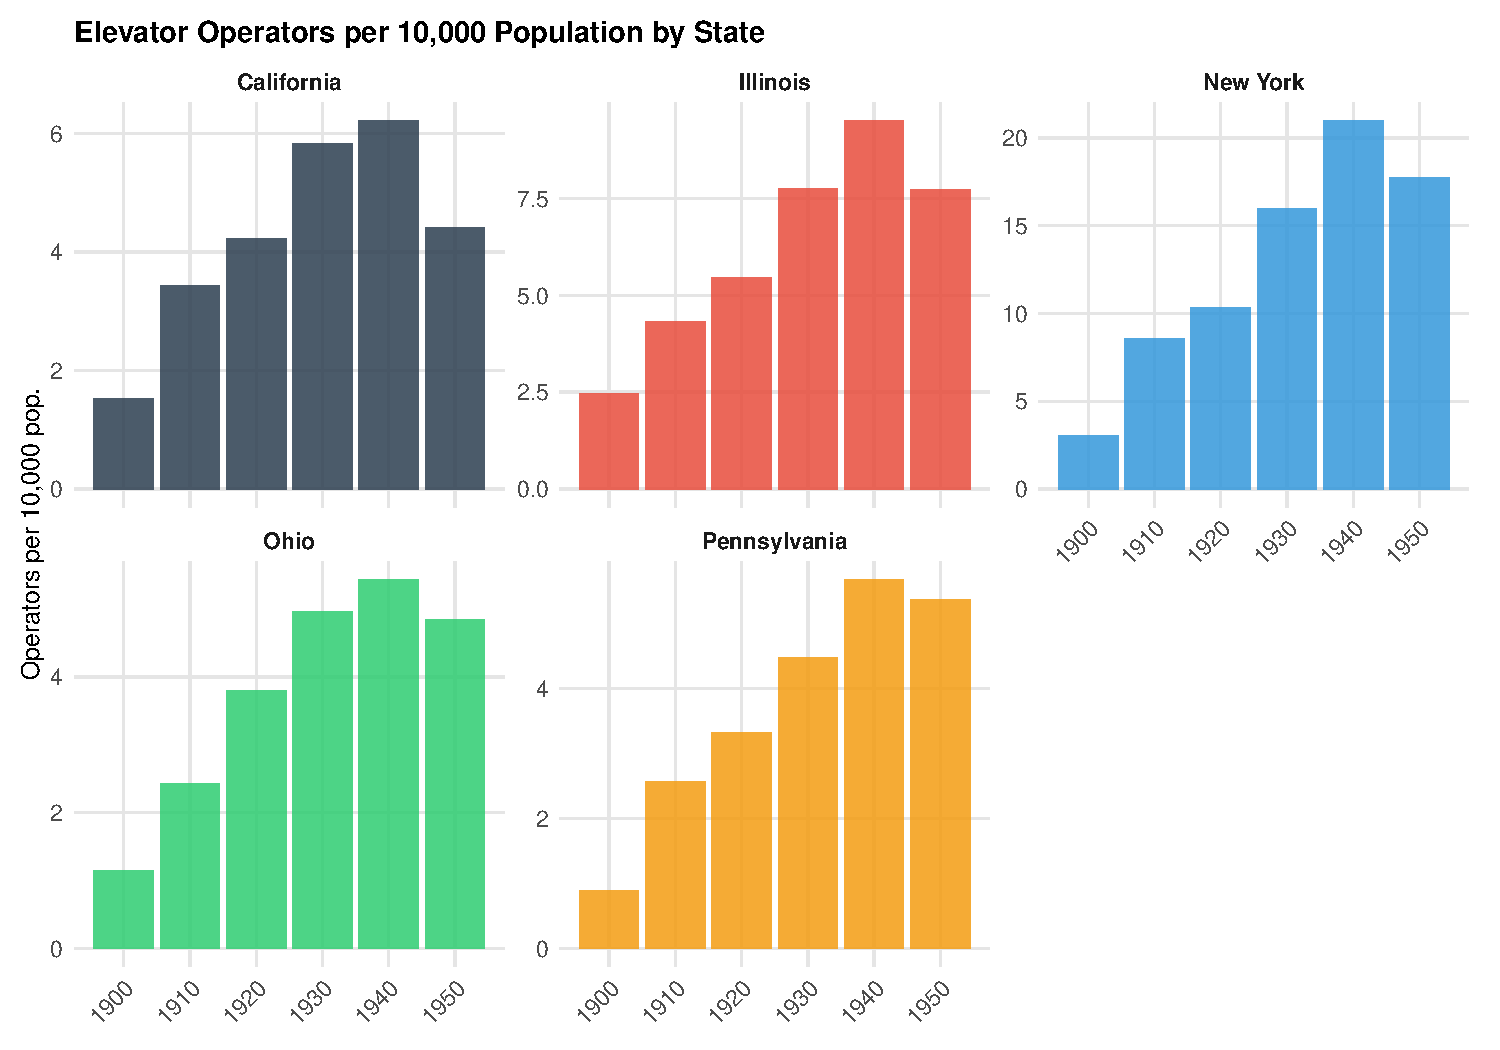
\includegraphics[width=0.85\textwidth]{figures/fig_a1_state_detail.pdf}
    \caption{Elevator Operators per 10,000 Population by State, 1900--1950}
    \label{fig:state_detail}
\end{figure}

\end{document}
